%Input preamble
%Style
\documentclass[12pt]{article}
\usepackage[top=1in, bottom=1in, left=1in, right=1in]{geometry}
\parindent 22pt
\usepackage{fancyhdr}

%Packages
\usepackage{adjustbox}
\usepackage{amsmath}
\usepackage{amsfonts}
\usepackage{amssymb}
\usepackage{bm}
\usepackage[table]{xcolor}
\usepackage{tabu}
\usepackage{color,soul}
\usepackage{makecell}
\usepackage{longtable}
\usepackage{multirow}
\usepackage[normalem]{ulem}
\usepackage{etoolbox}
\usepackage{graphicx}
\usepackage{tabularx}
\usepackage{ragged2e}
\usepackage{booktabs}
\usepackage{caption}
\usepackage{fixltx2e}
\usepackage[para, flushleft]{threeparttablex}
\usepackage[capposition=top,objectset=centering]{floatrow}
\usepackage{subcaption}
\usepackage{pdfpages}
\usepackage{pdflscape}
\usepackage{natbib}
\usepackage{bibunits}
\definecolor{maroon}{HTML}{990012}
\usepackage[colorlinks=true,linkcolor=maroon,citecolor=maroon,urlcolor=maroon,anchorcolor=maroon]{hyperref}
\usepackage{marvosym}
\usepackage{makeidx}
\usepackage{tikz}
\usetikzlibrary{shapes}
\usepackage{setspace}
\usepackage{enumerate}
\usepackage{rotating}
\usepackage{tocloft}
\usepackage{epstopdf}
\usepackage[titletoc]{appendix}
\usepackage{framed}
\usepackage{comment}
\usepackage{xr}
\usepackage{titlesec}
\usepackage{footnote}
\usepackage{longtable}
\newlength{\tablewidth}
\setlength{\tablewidth}{9.3in}
\setcounter{secnumdepth}{4}

\titleformat{\paragraph}
{\normalfont\normalsize\bfseries}{\theparagraph}{1em}{}
\titlespacing*{\paragraph}
{0pt}{3.25ex plus 1ex minus .2ex}{1.5ex plus .2ex}
\makeatletter
\pretocmd\start@align
{%
  \let\everycr\CT@everycr
  \CT@start
}{}{}
\apptocmd{\endalign}{\CT@end}{}{}
\makeatother
%Watermark
\usepackage[printwatermark]{xwatermark}
\usepackage{lipsum}
\definecolor{lightgray}{RGB}{220,220,220}
%\newwatermark[allpages,color=lightgray,angle=45,scale=3,xpos=0,ypos=0]{Preliminary Draft}

%Further subsection level
\usepackage{titlesec}
\setcounter{secnumdepth}{4}
\titleformat{\paragraph}
{\normalfont\normalsize\bfseries}{\theparagraph}{1em}{}
\titlespacing*{\paragraph}
{0pt}{3.25ex plus 1ex minus .2ex}{1.5ex plus .2ex}

\setcounter{secnumdepth}{5}
\titleformat{\subparagraph}
{\normalfont\normalsize\bfseries}{\thesubparagraph}{1em}{}
\titlespacing*{\subparagraph}
{0pt}{3.25ex plus 1ex minus .2ex}{1.5ex plus .2ex}

%Functions
\DeclareMathOperator{\cov}{Cov}
\DeclareMathOperator{\corr}{Corr}
\DeclareMathOperator{\var}{Var}
\DeclareMathOperator{\plim}{plim}
\DeclareMathOperator*{\argmin}{arg\,min}
\DeclareMathOperator*{\argmax}{arg\,max}

%Math Environments
\newtheorem{theorem}{Theorem}
\newtheorem{claim}{Claim}
\newtheorem{condition}{Condition}
\renewcommand\thecondition{C--\arabic{condition}}
\newtheorem{algorithm}{Algorithm}
\newtheorem{assumption}{Assumption}
\renewcommand\theassumption{A--\arabic{assumption}}
\newtheorem{remark}{Remark}
\renewcommand\theremark{R--\arabic{remark}}
\newtheorem{definition}[theorem]{Definition}
\newtheorem{hypothesis}[theorem]{Hypothesis}
\newtheorem{property}[theorem]{Property}
\newtheorem{example}[theorem]{Example}
\newtheorem{result}[theorem]{Result}
\newenvironment{proof}{\textbf{Proof:}}{$\bullet$}

%Commands
\newcommand\independent{\protect\mathpalette{\protect\independenT}{\perp}}
\def\independenT#1#2{\mathrel{\rlap{$#1#2$}\mkern2mu{#1#2}}}
\newcommand{\overbar}[1]{\mkern 1.5mu\overline{\mkern-1.5mu#1\mkern-1.5mu}\mkern 1.5mu}
\newcommand{\equald}{\ensuremath{\overset{d}{=}}}
\captionsetup[table]{skip=10pt}
%\makeindex

\setlength\parindent{20pt}
\setlength{\parskip}{0pt}

\newcolumntype{L}[1]{>{\raggedright\let\newline\\\arraybackslash\hspace{0pt}}m{#1}}
\newcolumntype{C}[1]{>{\centering\let\newline\\\arraybackslash\hspace{0pt}}m{#1}}
\newcolumntype{R}[1]{>{\raggedleft\let\newline\\\arraybackslash\hspace{0pt}}m{#1}}



%Logo
%\AddToShipoutPictureBG{%
%  \AtPageUpperLeft{\raisebox{-\height}{
\includegraphics[width=1.5cm]{uchicago.png}}}
%}

\newcolumntype{L}[1]{>{\raggedright\let\newline\\\arraybackslash\hspace{0pt}}m{#1}}
\newcolumntype{C}[1]{>{\centering\let\newline\\\arraybackslash\hspace{0pt}}m{#1}}
\newcolumntype{R}[1]{>{\raggedleft\let\newline\\\arraybackslash\hspace{0pt}}m{#1}}

\newcommand{\mr}{\multirow}
\newcommand{\mc}{\multicolumn}

%\newcommand{\comment}[1]{}

%Other parameters
\newcommand{\noutcomes}{95}
\newcommand{\noutcomesexpp}{357}
\newcommand{\noutcomesexpm}{343}
\newcommand{\noutcomesexpf}{355}
\newcommand{\treatsubsabc}{$75\%$}
\newcommand{\treatsubscarec}{$74\%$}
\newcommand{\treatsubscaref}{$63\%$}

%Counts
%Males
\newcommand{\positivem}{$78\%$}
\newcommand{\positivesm}{$29\%$}

%Females
\newcommand{\positivef}{$78\%$}
\newcommand{\positivesf}{$31\%$}

%Counts, control substitution
%Males
\newcommand{\positivecsnm}{$47\%$}
\newcommand{\positivescsnm}{$15\%$}

\newcommand{\positivecsam}{$79\%$}
\newcommand{\positivescsam}{$29\%$}

%Females
%% no alternative
\newcommand{\positivecsnf}{$84\%$}
\newcommand{\positivescsnf}{$55\%$}

%% alternative
\newcommand{\positivecsaf}{$79\%$}
\newcommand{\positivescsaf}{$33\%$}

%Pooled

%Effects
%Males

%Females
\newcommand{\empf}{$8$}
\newcommand{\yearsedf}{$1.7$}



%Pooled

%CBA
%IRR
%Males
\newcommand{\irrm}{$15\%$}
\newcommand{\irrsem}{$5\%$}

%Females
\newcommand{\irrf}{$9\%$}
\newcommand{\irrsef}{$7\%$}

%Pooled
\newcommand{\irrp}{$13\%$}
\newcommand{\irrsep}{$5\%$}

%BC
%Males
\newcommand{\bcm}{$11.24$}
\newcommand{\bcsem}{$4.60$}

%Females
\newcommand{\bcf}{$2.35$}
\newcommand{\bcsef}{$1.09$}

%Pooled
\newcommand{\bcp}{$5.63$}
\newcommand{\bcsep}{$2.15$}

%NPV streams
%Pooled
\newcommand{\parincomenpvp}{$\$119,346$}

\usepackage[stable]{footmisc}

\newcommand*\leftright[2]{%
  \leavevmode
  \rlap{#1}%
  \hspace{0.5\linewidth}%
  #2}

\newcommand{\orth}{\ensuremath{\perp\!\!\!\perp}}%
\newcommand{\indep}{\orth}%
\newcommand{\notorth}{\ensuremath{\perp\!\!\!\!\!\!\diagup\!\!\!\!\!\!\perp}}%
\newcommand{\notindep}{\notorth}

\externaldocument{abc_comprehensivecba_appendix-pub}
\externaldocument{abc_comprehensivecba_appendix-priv}
\pagenumbering{roman}

\begin{document}

\begin{titlepage}
\newgeometry{top=.8in, bottom=.8in, left=.8in, right=.8in}

\title{\Large \textbf{The Life-cycle Benefits \\ of an Influential Early Childhood Program}\thanks{This research was supported in part by the American Bar Foundation; the Pritzker Children's Initiative, the Buffett Early Childhood Fund; National Institutes of Health grants NICHD R37HD065072, NICHD R01HD54702, NIA R24AG048081, and P30AG024968; an anonymous funder; Successful Pathways from School to Work, an initiative of the University of Chicago's Committee on Education funded by the Hymen Milgrom Supporting Organization; and the Human Capital and Economic Opportunity Global Working Group, an initiative of the Center for the Economics of Human Development, affiliated with the Becker Friedman Institute for Research in Economics, and funded by the Institute for New Economic Thinking. The views expressed in this paper are solely those of the authors and do not necessarily represent those of the funders or the official views of the National Institutes of Health. The authors wish to thank Frances Campbell, Craig and Sharon Ramey, Margaret Burchinal, Carrie Bynum, and the staff of the Frank Porter Graham Child Development Institute at the University of North Carolina Chapel Hill for the use of data and source materials from the Carolina Abecedarian Project and the Carolina Approach to Responsive Education. We also thank the researchers of the HighScope Educational Research Foundation's Perry Preschool Study, especially Lawrence Schweinhart and Cheryl Polk, for access to study data and source materials. Years of partnership and collaboration with these project teams have made this work possible. Collaboration with Andr\'{e}s Hojman, Yu Kyung Koh, Sylvi Kuperman, Stefano Mosso, Rodrigo Pinto, Joshua Shea, Jake Torcasso, and Anna Ziff on related work has strengthened the analysis in this paper. Collaboration with Bryan Tysinger of the Leonard D. Schaeffer Center for Health Policy and Economics at the University of Southern California on adapting the Future America Model is gratefully acknowledged. For helpful comments on various versions of the paper, we thank St\'{e}phane Bonhomme, Fl\'{a}vio Cunha, Steven Durlauf, Dana Goldman, Sidharth Moktan, Azeem Shaikh, Matthew Tauzer, and Ed Vytlacil. We also benefited from helpful comments received at a Russell Sage Foundation seminar in September, 2016. For information on the implementation of the Carolina Abecedarian Project and the Carolina Approach to Responsive Education and assistance in data acquisition, we thank Peg Burchinal, Carrie Bynum, Frances Campbell, and Elizabeth Gunn. For information on childcare in North Carolina, we thank Richard Clifford and Sue Russell. The set of codes to replicate the computations in this paper are posted in a repository. Interested parties can request to download all the files except for those of the Future America Model, due to private interests. The address of the repository is \url{https://github.com/jorgelgarcia/abccare-cba}. Data agreements do not allow us to post some of the data files that we use. Interested parties can contact any of the authors to be given a temporary license to access the data and replicate the results. The Web Appendix for this paper is posted on \url{http://cehd.uchicago.edu/ABC_CARE}.}}

\author{
Jorge Luis Garc\'{i}a\\
Department of Economics\\
The University of Chicago \and
James J. Heckman \\
American Bar Foundation \\
Department of Economics\\
The University of Chicago \and
Duncan Ermini Leaf \\
Leonard D. Schaeffer Center \\  for Health Policy and Economics\\
University of Southern California \and
Mar\'{i}a Jos\'{e} Prados \\
Dornsife Center for \\ Economic and Social Research\\
University of Southern California}
\date{First Draft: January 5, 2016\\ This Draft: \today}

\maketitle
\restoregeometry
\end{titlepage}

\singlespacing
\begin{abstract}
\noindent This paper estimates the large array of long-run benefits of an influential early childhood program targeted to disadvantaged children and their families. It is evaluated by random assignment and follows participants through their mid-30s. The program is a prototype for numerous interventions currently in place around the world. It has substantial beneficial impacts on (a) health and the quality of life, (b) the labor incomes of participants, (c) crime, (d) education, and (e) the earnings of the mothers of the participants through subsidizing their childcare. There are substantially greater monetized benefits for males. The overall rate of return is a statistically significant 12.3\% per annum with an associated benefit/cost ratio of 5.7. These estimates account for the welfare costs of taxation to finance the program. They survive a variety of sensitivity analyses. Accounting for substitutes to treatment available to families randomized out of treatment shows that boys benefit much less than girls from low quality alternative childcare arrangements.
\end{abstract}

\noindent \textbf{Keywords}: Childcare, early childhood education, gender differences in responses to programs, health, long-term predictions, quality of life, randomized trials, substitution bias \\
\noindent \textbf{JEL codes}: J13, I28, C93

\bigskip

\begin{tabular}{ll}
Jorge Luis Garc\'{i}a                                       & James J. Heckman \\
Department of Economics                                & Department of Economics \\
University of Chicago                                       & University of Chicago \\
1126 East 59th Street                                     & 1126 East 59th Street \\
Chicago, IL 60637                                           & Chicago, IL 60637 \\
Phone: 773-677-7938                                     & Phone: 773-702-0634  \\
Email: jorgelgarcia@uchicago.edu                       & Email: jjh@uchicago.edu \\
                                                                       & \\
Duncan Ermini Leaf                                           & Mar\'{i}a Jos\'{e} Prados \\
Leonard D. Schaeffer Center for            & Dornsife Center for  \\
Health Policy \& Economics                                          & Economic and Social Research \\
University of Southern California                        & University of Southern California \\
635 Downey Way                                             & 635 Downey Way        \\
Los Angeles, CA 90089                                    & Los Angeles, CA 90089 \\
Phone: 213-821-6474                                     & Phone: 213-821-7969 \\
Email: dleaf@healthpolicy.usc.edu                     & Email: prados@usc.edu \\

\end{tabular}


\clearpage

\restoregeometry
\doublespacing

\setcounter{page}{0}
\pagenumbering{arabic}

\section{Introduction}

This paper documents the large array of life-cycle benefits of an influential early childhood program targeted to disadvantaged children. The program has substantial impacts on the lives of participants. Monetizing benefits and costs across multiple domains, we estimate a rate of return of 12.3\% per annum and a benefit/cost ratio of 5.7. There are substantial differences across genders favoring males.

Our analysis contributes to a growing literature on the value of early programs for disadvantaged children.\footnote{See, e.g., \cite{Currie_2011_AER} and \cite{Elango_Hojman_etal_2016_Early-Edu}.} Long-term evidence on their effectiveness is surprisingly limited.\footnote{The major source of evidence is from the Perry Preschool Program (see \citealp{Schweinhart_Montie_ea_2005_BOOKlifetime} and \citealp{Heckman_Moon_etal_2010_RateofReturn,Heckman_Moon_etal_2010_QE}), the Carolina Abecedarian Project (ABC) and the Carolina Approach to Responsive Education (CARE) (\citealp{Ramey_Campbell_etal_2000_ADS,Ramey-etal_2012-ABC}), and the Infant Health and Development Program (IHDP) (\citealp{Gross_Spiker_etal_1997_BOOKHelpinglowbirth,Duncan_Sojourner_2013_JHR}). IHDP was inspired by ABC/CARE \citep[][]{Gross_Spiker_etal_1997_BOOKHelpinglowbirth}.} For want of follow-up data, many studies of early childhood programs report only a few early age outcomes like IQ or scores on school readiness measures.\footnote{See, e.g., \cite{Kline_Walters_2016_QJE} and \cite{Weiland_2013_CD_Impacts-of-Pre-K}.} Yet it is the long-term returns that are relevant for policy analysis.

We analyze the costs and benefits from two virtually identical early childhood programs evaluated by randomized trials conducted in North Carolina. The programs are the Carolina Abecedarian Project (ABC) and the Carolina Approach to Responsive Education (CARE) -- henceforth ABC/CARE. Both were launched in the 1970s and have long-term follow-ups through age 34. The programs started early (at 8 weeks of life) and engaged participants to age 5. We analyze their impacts on a variety of life outcomes such as health, the quality of life,\footnote{Throughout this paper, \textit{we refer to health-related quality of life as quality of life}. It is the weight attached to each year of life as a function of disease burden, as we detail further below.} participation in crime, labor income, IQ, schooling, and increased parental earnings arising from subsidized childcare.\footnote{The income we observe is aggregated across the parents. Only 27\% of the mothers lived with a partner at baseline, so we refer to the gain in parental income as a gain in mother's labor income.}

Evidence from these programs is relevant for contemporary policy discussions because their main components are present in a variety of current interventions.\footnote{Programs inspired by ABC/CARE have been (and are currently being) launched around the world. \citet{Sparling_2010_Highlights} and \citet{Ramey_Ramey_Lanzi_2014_Interventions} list numerous programs based on the ABC/CARE approach. The programs are, with years launched and locations in parentheses: IHDP---eight different cities around the U.S. \citep{Spiker-etal_1997_Helping}; Early Head Start and Head Start in the U.S. \citep{Schneider_McDonald-eds_2007_Scale-Up_Vol-1}; John's Hopkins Cerebral Palsy Study in the U.S. \citep{Sparling_2010_Highlights}; Classroom Literacy Interventions and Outcomes (CLIO) study in the U.S. \citep{Sparling_2010_Highlights}; Massachusetts Family Child Care Study \citep{Collins_etal_2010_Massachusetts-Study}; Healthy Child Manitoba Evaluation \citep{Healthy_Child_Manitoba_2015_Starting-Early}; Abecedarian Approach within an Innovative Implementation Framework \citep{Jensen_Nielsen_2016_ABC-Programme-Pilot}; and Building a Bridge into Preschool in Remote Northern Territory Communities in Australia \citep{UMonash_Dataset_2015_URL}. Educare programs are also based on ABC/CARE \citep{Educare_2014_Research_Agenda,Yazejian_Bryant_2012_Educare}.} About 19\% of all African-American children are eligible for these programs today.\footnote{43\% of African-American children were eligible in 1972.}

Analyzing the benefits of programs with a diverse array of outcomes across multiple domains and periods of life is both challenging and rewarding. Doing so highlights the numerous ways through which early childhood programs enhance adult capabilities. We use a variety of measures to characterize program benefits. Instead of reporting only individual treatment effects or categories of treatment effects, our benefit/cost analyses account for all measured aspects of these programs, including the welfare costs of taxes to publicly finance them. We display the sensitivity of our estimates excluding various components of costs and benefits.\footnote{\cite{Barnett_Masse_2002_benefitcost,Barnett_Masse_2007_EER} present a cost/benefit analysis for ABC through age 21, before many benefits are realized. They report a benefit/cost ratio of 2.5, but give no standard error or sensitivity analyses for their estimate. They do not disaggregate by gender. For want of the data collected on health at age 34, they do not account for health benefits. They use self-reported crime data (unlike the administrative crime data later collected that we analyze) and ignore the welfare costs of financing the program. We use cost data from primary sources not available to them.}

A fundamental problem in evaluating any intervention is assessing out-of-sample future benefits. Solutions to this problem are based on versions of a synthetic cohort approach using the outcomes of older cohorts not eligible for the program who are otherwise comparable to treated and control persons to proxy future treatment effects.\footnote{\cite{Mincer_1974_schooling} addresses this problem using a synthetic cohort approach and provides evidence on its validity. See the discussion of the synthetic cohort approach in \cite{Heckman_Lochner_ea_2006_HEE}.} Using this approach, we combine experimental data through age 34 with information from multiple auxiliary panel data sources to predict benefits and costs over the lifetimes of participants.\footnote{\citet{Ridder_Moffitt_2007_hbk_metricsdata} provide a valuable discussion of data combination methods. These methods are related to the older ``surrogate marker'' literature in biostatistics (see e.g., \citealp{Prentice_1989_Surrogate_SiM}).}

Our analysis is simplified by the finding that all eligible families offered participation in the program take the offer. This motivates a revealed preference approach to constructing synthetic control groups. We develop a synthetic treatment group drawing on the analysis of \citet{Heckman_Pinto_etal_2013_PerryFactor}. They show that program treatment effects are produced through changes in inputs in a stable (across treatment regimes) production function for outcomes. We use the estimated production function to make out-of-sample predictions based on inputs caused by treatment.

We account for sampling uncertainty arising from combining data, estimating parameters of behavioral equations, and simulating models. We conduct sensitivity analyses for outcomes for which sampling uncertainty is not readily quantified. Our approach to combining multiple data sets and analyzing blocks of outcomes is of interest in its own right as a template for evaluating other programs with numerous long-run outcomes using intermediate outcome measures.

Our analysis accounts for control group substitution.\footnote{See \cite{Heckman_1992_randomization}, \cite{Heckman_Hohmann_etal_2000_QJE}, and \cite{Kline_Walters_2016_QJE}.} Roughly 75\% of the control-group children in ABC/CARE enroll in some form of lower quality alternative childcare outside of the home.\footnote{We refer to alternatives as alternative childcare or alternative preschool centers. See Appendix~\ref{appendix:background} for a precise description of these alternatives.} We define and estimate parameters accounting for the choices taken by the control groups in our study.

We find pronounced gender differences in treatment effects comparing high quality treatment with lower quality alternatives. Males benefit much less from alternative market childcare arrangements compared to females, a result consistent with the literature on the vulnerability of male children when removed from their mothers, even for short periods.\footnote{See \citet{Kottelenberg-Lehrer_2014_Gender-Effects} and \citet{Baker_Gruber_Milligan_2015_Noncog_Defects}.}

We contribute to the literature on the effectiveness of early childhood programs by considering their long-term benefits on health. We estimate the savings from life-cycle medical costs and from improvements in the quality of life.\footnote{\cite{Campbell_Conti_etal_2014_EarlyChildhoodInvestments} show the substantial adult (age 34) health benefits of ABC but do not present a cost/benefit analysis of their results.} We find substantial childcare benefits that promote work by the mothers of participants, and additional benefits for participants in terms of reduced crime, gains in life-cycle labor income, reduced special education costs and enhanced educational attainment.

Figure~\ref{figure:main} summarizes the main findings of this paper. It displays the discounted (by a 3\% discount rate) life-cycle benefits of the program and costs (in 2014 USD) for a pooled sample of male and female participants, overall and disaggregated by category. We also report separate estimates by gender. Costs are substantial, as has frequently been noted by critics.\footnote{See, e.g., \citet{Whitehurst_2014_Senate_Testimony} and \citet{Fox_News_2014_Head_Start_Effects}.} But so are the benefits, which far outweigh the costs.

\begin{sidewaysfigure}[!htbp]
\caption{Net Present Value of Main Components of the Cost/Benefit Analysis Over the Life Cycle per Program Participant, Treatment vs. Next Best}\label{figure:main}
\centering
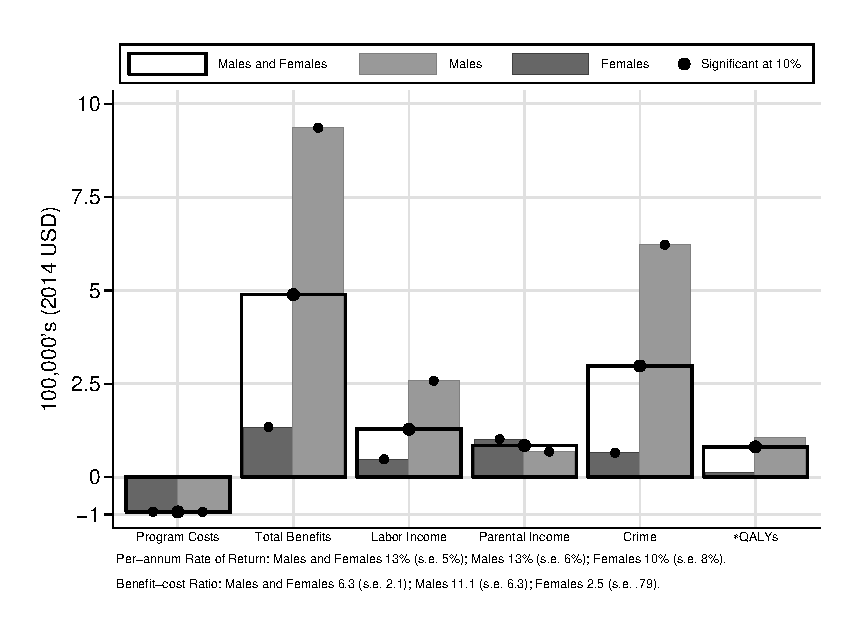
\includegraphics[width=.7\columnwidth]{output/abccare_npvssumm.eps}
\floatfoot{
\footnotesize
Note: This figure displays the life-cycle net present values per program participant of the main components of the cost/benefit analysis of ABC/CARE from birth to predicted death, discounted to birth at a rate of 3\%.  By ``net" we mean that each component represents the total value for the treatment group minus the total value for the control group. Program costs: the total cost of ABC/CARE, including the welfare cost of taxes to finance it. Total net benefits: for \textit{all} of the components we consider. These include labor income: total individual labor income from ages 20 to the retirement of program participants (assumed to be at age 67). Parental income: total parental labor income of the parents of the participants from when the participants were ages 1.5 to 21. Crime: the total cost of crime (judicial and victimization costs). To simplify the display , the following components are not shown in the figure: (i) cost of alternative preschool paid by the control group children parents; (ii) the social welfare costs of transfer income from the government; (iii) disability benefits and social security claims; (iv) costs of increased individual and maternal education (including special education and grade retention); (v) total medical public and private costs. Inference is based on non-parametric, one-sided $p$-values from the empirical bootstrap distribution. We indicate point estimates significant at the $10\%$ level.\\
*QALYs refers to the quality-adjusted life years. Any gain corresponds to better health conditions until predicted death, with $\$150,000$ (2014 USD) as base value for a year of life.\\}
\end{sidewaysfigure}

The rest of the paper justifies and interprets these estimates. We proceed in the following way. Section~\ref{section:background} discusses the ABC/CARE intervention. Section~\ref{section:methodsquestions} presents our notation and the definitions of the treatment effects estimated in this paper. Section~\ref{section:methodology} discusses our approaches to inference for vectors of treatment effects. We use combining functions that summarize the \emph{number} of beneficial outcomes, as well as the number of statistically significant beneficial outcomes.

Section~\ref{section:c-functions} reports estimated treatment effects. Section~\ref{section:cbamethodology} presents our approaches for predicting life-cycle outcomes and evidence supporting the assumptions underlying it. Section~\ref{section:cbaresults} reports our estimates of benefit/cost ratios and rates of return. Section~\ref{section:conclusion} summarizes the paper.

As is evident from Figure~\ref{figure:main}, there are substantial benefits that differ by gender. Girls benefit across more domains. However, the monetized value of the estimated treatment effects is substantially greater for boys. This discrepancy is largely driven by labor income and health benefits, as well as reduced crime for males. Males benefit much less than females from being placed in lower quality alternative early childcare programs, compared to remaining with their mothers at home.

\section[Background and Data Sources]{Background and Data Sources} \label{section:background}

\subsection{Overview}

ABC/CARE targeted disadvantaged, predominately African-American children in Chapel Hill/Durham, North Carolina.\footnote{Both ABC and CARE were designed and implemented by researchers at the Frank Porter Graham Center of the University of North Carolina in Chapel Hill.} Table~\ref{tab:programcomparison} compares the two virtually identical programs. Appendix~\ref{appendix:background} describes these programs in detail. Here, we summarize their main features.

The goal of these programs was to enhance the early-life skills of disadvantaged children. Both programs supported language, motor, and cognitive development as well as socio-emotional competencies considered crucial for school success including task-orientation, ability to communicate, independence, and pro-social behavior.\footnote{\citet{Ramey_Collier_etal_1976_CarolinaAbecedarianProject, Ramey_etal_1985_Project-CARE_TiECSE, Sparling_1974_Synth_Edu_Infant_SPEECH, Wasik_Ramey_etal_1990_CD, Ramey-etal_2012-ABC}.}

The programs individualized treatment. Each child's progress was recorded and learning activities were appropriately adjusted every 2 to 3 weeks. Environments were organized to promote pre-literacy and access to a rich set of learning tools.\footnote{The ``LearningGames'' approach was implemented by infant and toddler caregivers in 1:1 child-adult interactions. Each ``LearningGames'' activity states a developmentally-appropriate objective, the necessary materials, directions for teacher behavior, and expected child outcome.} The curriculum emphasized active learning experiences, dramatic play, and basic concepts of order and category (``pre-academic skills''), as well as discipline and the ability to interact with and respect others.  At later ages (3 through 5), the program focused on the development of ``socio-linguistic and communicative competence.''\footnote{\citet{Ramey-et-al_1977_Intro-to-ABC, Haskins_1985_CD, Ramey_1981_Modification, Ramey_Campbell_1979_SR, Ramey_Smith_1977_AJMD, Ramey_McGinness_etal_1982_Abecedarianapproach, Sparling_Lewis_1979_BOOKLearninggamesFirstThree,Sparling_Lewis_1984_BOOKLearningGamesThreesFours}.}

ABC recruited four cohorts of children born between 1972 and 1976. CARE recruited two cohorts of children, born between 1978 and 1980. The recruitment processes for each study were identical. Potential participant families were referred to researchers by local social service agencies and hospitals at the beginning of the mother's last trimester of pregnancy. Eligibility was determined by a score on a childhood risk index.\footnote{See Appendix~\ref{appendix:background} for details on the construction for the index used. The index weighs the following variables (listed from the most to the least important according to the index): maternal and paternal education, family income, father's presence at home, lack of maternal relatives in the area, siblings behind appropriate grade in school, family in welfare, father in unstable job, maternal IQ, siblings' IQ, social agency indicates that the family is disadvantaged, one or more family members has sought a form of professional help in the last three years, and any other special circumstance detected by program's staff.}

As shown in Table~\ref{tab:programcomparison}, the design and implementation of ABC and CARE were very similar. ABC had two phases, the first of which lasted from birth until age 5. In this phase, children were randomly assigned to treatment. The second phase of the study consisted of child academic support through home visits from ages 5 through 8. CARE consisted of two treatment phases as well, very similar to ABC. The first phase of CARE from birth until age 5, had an additional treatment arm of home visits designed to improve home environments.\footnote{\citet{Wasik_Ramey_etal_1990_CD}.} Participation in the second phase was randomized in ABC, but not in CARE.

Our analysis is based on the first phase and pools the treatment group in CARE with the ABC treatment group. The second-phase treatment of ABC/CARE had little impact on participants (for evidence, see \citealp{Campbell_Conti_etal_2014_EarlyChildhoodInvestments} and \citealp{ABCCARE_Dataset}). \citet{Campbell_Conti_etal_2014_EarlyChildhoodInvestments} establish the validity of pooling the data on second phase treatments and controls with the first phase controls in ABC.

We do not use the data on the CARE group that only received home visits in the early years. \citet{Campbell_Conti_etal_2014_EarlyChildhoodInvestments} and \citet{ABCCARE_Dataset} show that there is no statistically significant effect of this component.

\begin{table}[!htbp]
\centering
\caption{ABC and CARE, Program Comparison} \label{tab:programcomparison}
\begin{adjustbox}{max width=\textwidth}
\begin{threeparttable}
	\small
	\begin{table}[H]
\begin{center}
\begin{threeparttable}
\caption{ABC and CARE, Programs Comparison} \label{tab:programcomparison}
\scriptsize
\scalebox{.9}{\begin{tabular}{L{4cm} L{7cm} L{5cm}}
\hline \hline
& \multicolumn{1}{c}{ABC}& \multicolumn{1}{c}{CARE}\\
\hline 
Program Overview &&\\
\hspace{.5cm} Years Implemented &1972--1982&1978--1985\\
\hspace{.5cm} Age of Entry/Exit & birth to 5 years old &\checkmark\\
\hspace{.5cm} Initial Sample &122&64\\
\hspace{.5cm} \# of Cohorts &4&2\\
\midrule
Eligibility & socio-economic disadvantage according to a multi-factor index (see Section \ref{section:eligibility})&\checkmark\\
 \midrule
Control &&\\
\hspace{.5cm} N &54&23\\
\hspace{.5cm} Compensation & Diapers from birth to age 3, unlimited formula from birth to 15 months & \checkmark \\
\hspace{.5cm} Treatment Substitution & 70\% & $\sim$ 70\%\\
\midrule
Treatment & Center-based childcare & Center-based childcare and family education\\
\hspace{.5cm} \textbf{Center-base} &&\\
\hspace{.5cm} \textbf{Childcare} &&\\
\hspace{.5cm} N &57&17\\
\hspace{.5cm} Intensity &6.5--9.75 hours a day for 50 weeks per year&\checkmark\\
\hspace{.5cm} Components & Instruction, medical care, nutrition, social services &\checkmark\\
\hspace{.5cm} Staff-to-child Ratio &1:3 during ages 0--1 &\checkmark\\
&1:4--5 during age 1--4 &\checkmark\\&1:5--6 during ages 4--5 &\checkmark\\
\hspace{.5cm} Staff Qualifications &Mixed diplomas; experienced&\checkmark\\
\hspace{.5cm} \textbf{Family Education} & Not part of the program &24\\
\hspace{.5cm} Intensity && One hour-long home visits. 2--3 per month during ages 0--3. 1--2 per month during ages 4--5\\
\hspace{.5cm} Curriculum & & Social and mental stimulation; parent-child interaction\\
\hspace{.5cm} Staff-to-child Ratio &&1:1\\
\hspace{.5cm} Staff Qualifications &&Home visitor training\\
\midrule
 School-age Treatment \\
 \hspace{.5cm} N&46&39\\
\hspace{.5cm} Intensity &Every other week& \checkmark\\
\hspace{.5cm} Components &Parent-teacher meetings& \checkmark\\
\hspace{.5cm} Curriculum & Reading and math &\checkmark\\
\hspace{.5cm} Staff-to-child Ratio &1:1&\checkmark\\
\hspace{.5cm} Staff Qualifications &Graduate degree and training in special education & \checkmark\\
\midrule
Data Availability \\
Questionnaires & Ages 0--5, 8, 12, 15, 21, 30--34 & Ages 0--5, 8, 12, 21, 30--34 \\
Parent Interview & Ages 0--5, 8, 12, 15, 21& Ages 0--5, 9, 12 \\  
Health Follow-up & Ages 30--34&\checkmark\\
\hline \hline
\end{tabular}}
\footnotesize
\begin{tablenotes}
\item Note: This table compares the main elements of ABC and CARE, summarized within this section.
\end{tablenotes}
\end{threeparttable}
\end{center}
\end{table}
\begin{tablenotes}
\small
\item Note: This table compares the main elements of ABC and CARE, summarized in this section. A \checkmark\ indicates that ABC and CARE had the same feature. A blank space indicates that the indicated component was not part of the program.
\end{tablenotes}
\end{threeparttable}
\end{adjustbox}
\end{table}

For both programs, from birth until the age of 8, data were collected annually on cognitive and socio-emotional skills, home environments, family structure, and family economic characteristics. After age 8, data on cognitive and socio-emotional skills, education, and family economic characteristics were collected at ages 12, 15, 21, and 30.\footnote{At age 30, measures of cognitive skills are unavailable for both ABC and CARE.} In addition, we have access to administrative criminal records and a physician-administered medical survey at age 34. This allows us to study the long-term effects of the programs along multiple dimensions of human development.\footnote{See Appendix~\ref{appendix:data} for a more comprehensive description of the data. There, we document the balance in observed baseline characteristics across the treatment and control groups, once we drop the individuals for whom we have no crime or health information, for which there is substantial attrition. Further, the methodology we propose addresses missing data in either of these two outcome categories.}

\subsection{Randomization Protocol and Compromises} \label{section:randomization}

Randomization for ABC/CARE was conducted on child pairs matched on family background. Siblings and twins were jointly randomized into either treatment or control groups.\footnote{For siblings, this occurred when two siblings were close enough in age such that both of them were eligible for the program.} Randomization pairing was based on a risk index, maternal education, maternal age, and gender of the subject.\footnote{We do not know the original pairs.} ABC collected an initial sample of 122 subjects. We characterize each missing observation in Appendix~\ref{appendix:background}. In Appendix~\ref{app:method_partialobs}, we document that our estimates are robust when we adjust for missing data using standard methods. We conduct the same analysis for the CARE sample. 22 subjects in ABC did not stay in the program through age 5. Dropouts are evenly balanced and are primarily related to the health of the child and mobility of families and not to dissatisfaction with the program.\footnote{The 22 dropouts include four children who died, four children who left the study because their parents moved, and two children who were diagnosed as developmentally delayed. Details are in Table~\ref{table:abccompromises}. Everyone offered the program was randomized to either treatment or control. All eligible families agreed to participate. Dropping out occurs \emph{after} randomization.}

\subsection{Control Group Substitution}

In ABC/CARE, many control group members (but no family offered treatment) attended alternative (to home) childcare or preschool centers.\footnote{See \cite{Heckman_Hohmann_etal_2000_QJE} on the issue of substitution bias in social experiments.} The figure is \treatsubsabc\ for ABC and \treatsubscarec\ for CARE. Figure~\ref{fig:salmonella} shows enrollment by age and the average months of enrollment by age for the control-group children who enrolled in program alternatives. Enrollment increases with the age of children.

\begin{sidewaysfigure}[!htbp]
\centering
\caption{Control Substitution Characteristics, ABC/CARE Control Group}\label{fig:control-sub}
\begin{subfigure}[h]{0.4\textwidth}
	\centering
	\caption{Enrollment by Age} \label{fig:salmonella}
		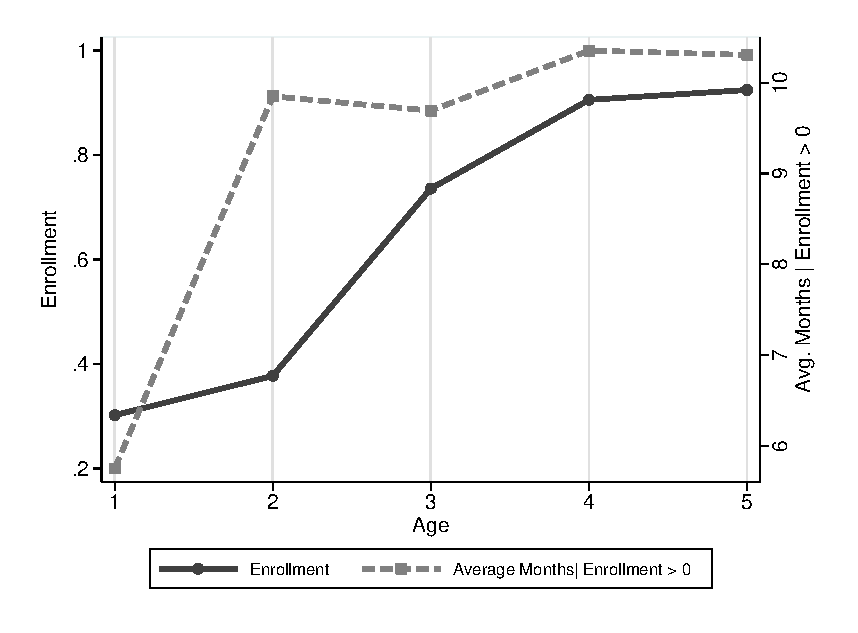
\includegraphics[width=\textwidth]{output/abccare_Valtenrollment.eps}
\end{subfigure}
\begin{subfigure}[h]{0.4\textwidth}
		\centering
		\caption{Enrollment Dynamics} \label{fig:treatsubcare_2}
		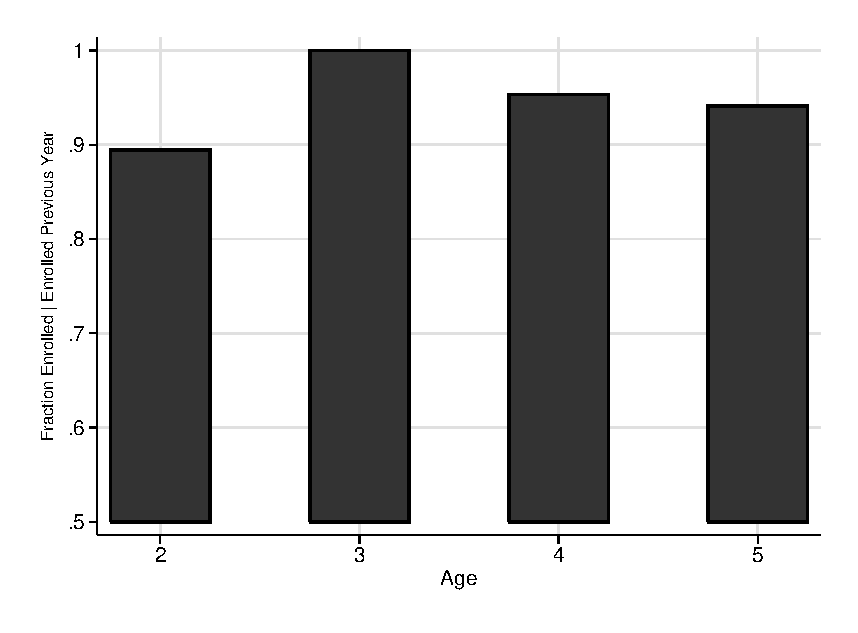
\includegraphics[width=\textwidth]{output/abccare_Vprobs.eps}
\end{subfigure}\\
\begin{subfigure}[h]{0.4\textwidth}
		\centering
		\caption{Cumulative Enrollment} \label{fig:treatsubcare}
		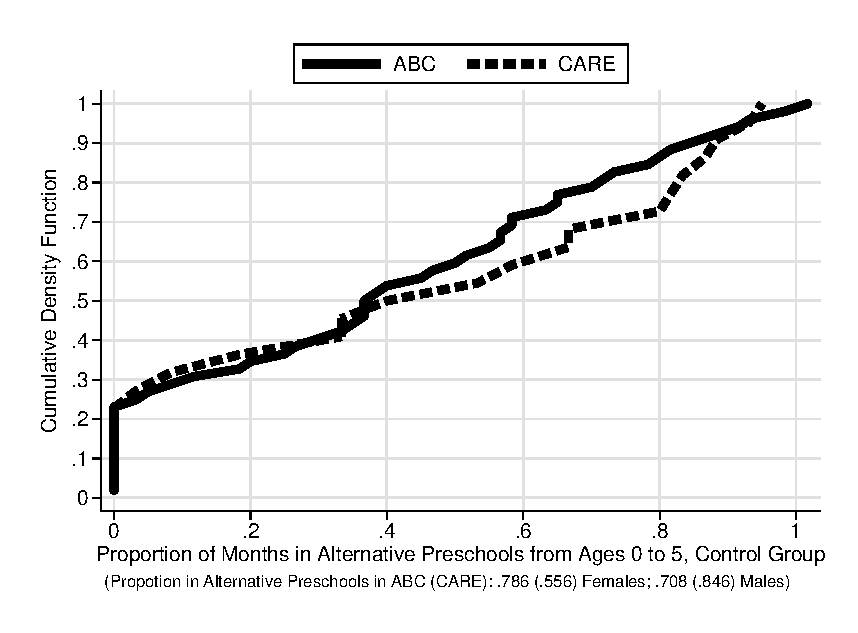
\includegraphics[width=\textwidth]{output/abccare_controlcontamination.eps}
\end{subfigure}
\begin{subfigure}[h]{0.4\textwidth}
	\centering
	\caption{Enrollment Intensity} \label{fig:proportion-alt-pre}
		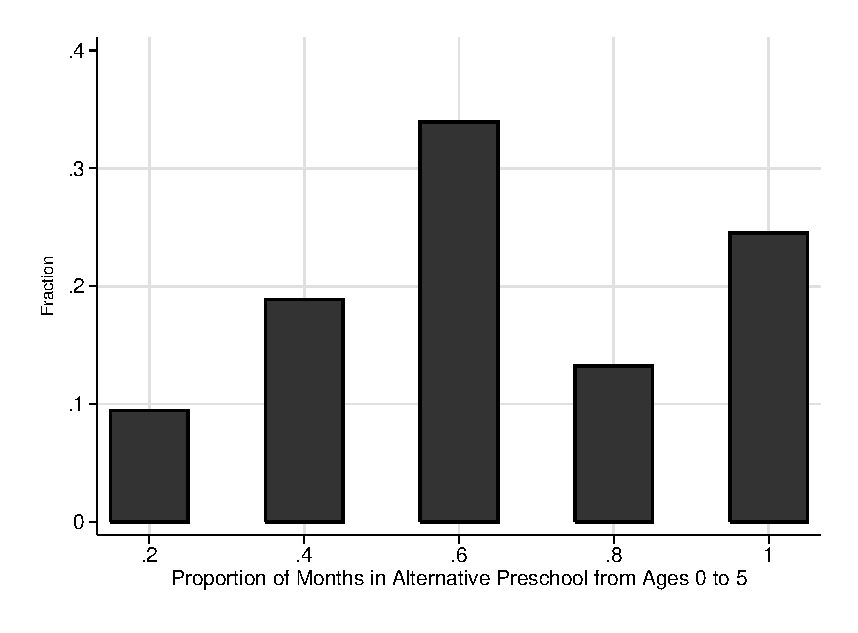
\includegraphics[width=\textwidth]{output/abccare_Vfractimes.eps}
\end{subfigure}%

\footnotesize \justify
Note: Panel (a) displays the fraction of the ABC/CARE control group enrolled in alternatives by age on the left axis and average number of months in alternative preschool by age in the right axis. Panel (b) displays the fraction of ABC/CARE control-group children enrolled in alternatives, conditional on being enrolled in the previous age (at least one month). Panel (c) displays the cumulative distribution function of enrollment in alternatives. Panel (d) displays the fraction of children in the ABC/CARE control groups enrolled in alternatives (fraction of children who were enrolled in alternatives 20\%, 40\%, 60\%, 80\%, and 100\% of the time, from ages 0 to 5). \\
\end{sidewaysfigure}

Figure~\ref{fig:treatsubcare_2} shows the proportion of the control sample enrolled in an alternative at a given age who persist in alternative care at the next age. Once enrolled, they generally stay enrolled and go for a full year.  Figure~\ref{fig:treatsubcare} shows (for each program) the cumulative distribution of the proportion of the first five years that control subjects were enrolled in alternatives. Figure~\ref{fig:proportion-alt-pre} shows the distribution of time spent in the alternative program for all control group participants.

Children in the control group who are enrolled in alternative early childcare programs are less economically disadvantaged at baseline compared to children who stay at home. Disadvantage is measured by maternal education, maternal IQ, Apgar scores at minutes 1 and 5, and the high-risk index defining ABC/CARE eligibility. Children who attend alternatives have fewer siblings. On average, they are children of mothers who are more likely to be working at baseline.\footnote{Statistically significant at 10\%.} Parents of girls are much more likely to use alternative childcare if assigned to the control group.\footnote{See Table~\ref{table:controlsubscharacteristics} in Appendix~\ref{appendix:background} for tests of differences across these variables between children in the control group who attend and who do not attend alternative preschools.}

Most of the alternative childcare centers received federal subsidies and were subject to the federal regulations of the era.\footnote{Appendix~\ref{appendix:tetanus} discusses the federal standards of that day. See \citet{Department-of-Health_1968_DayCareRequirements,NCGA_1971_House-Bill-100,Ramey-et-al_1977_Intro-to-ABC,Ramey_Campbell_1979_SR,Ramey_McGinness_etal_1982_Abecedarianapproach, Burchinal_Campbell_etal_1997_CD}.} They had relatively low quality compared to ABC/CARE.\footnote{When we compare ABC/CARE treatment to these alternatives, ABC/CARE has substantial treatment effects. Further, as we argue below, parents perceived that ABC/CARE was superior to the alternatives.} The access of control-group children to alternative programs affects the interpretation of estimated treatment effects, as we discuss next.

\section{The Parameters Estimated in This Paper} \label{section:methodsquestions}

Random assignment to treatment does not guarantee that conventional treatment effects answer policy-relevant questions. In this paper, we define and estimate three parameters that address different policy questions.

We assume that life cycles consist of $A$ discrete periods. The treatment phase is the first $\bar{a}$ periods of life $\left[1,\dots,\bar{a}\right]$. We have data through age $a^{*}>\bar{a}$. We lack follow-up data on the remainder of life $(\bar{a},\dots,A]$. We define $W=1$ to indicate that parents wish to participate in the program.\footnote{Individual subscripts are omitted to improve clarity.} We define $R \in \{0,1\}$, where $R=1$ indicates that a child is randomized into eligibility to participate in the program. $D$ indicates participation in the program.

Individuals are eligible to participate in the program if baseline background variables $\bm{B}\in\mathcal{B}_0$. $\mathcal{B}_0$ is the set of scores on a risk index required to be eligible, as previously discussed. As it turns out, in the ABC/CARE study, all of the eligible persons given the option to participate choose to do so $(W=1\text{, and } D=R)$.\footnote{There are no cases of non-compliance for people offered treatment, although there is a small amount of attrition. See Appendix~\ref{appendix:background} for details.} There are very few dropouts. \emph{Ex ante}, parents perceived that ABC/CARE was superior to other childcare alternatives. Thus, we can safely interpret the treatment effects generated by the experiment as average treatment effects for the population for which $\bm{B}\in\mathcal{B}_0$ and not just treatment effects for the treated (\textbf{TOT}).

Let $\bm{Y}^1_a$ be the outcome vector at age $a$ for the treated. $\bm{Y}^0_a$ is the age-$a$ outcome vector for the controls. In principle, life-cycle outcomes for the treatments and controls can depend on the exposures to various alternatives at each age. It would be desirable to estimate treatment effects for each possible exposure but our samples are too small to make credible estimates for very detailed exposures.

All treatment group children have the same exposure. We simplify the analysis of the controls by creating two categories. ``$H$'' indicates that the control child is in home care throughout the entire length of the program. ``$C$'' indicates that the control child is in an alternative childcare for any amount of time. We test the sensitivity of our estimates to the choice of different categorizations in our empirical analysis reported below.

We thus compress a complex reality into two counterfactual outcome states at age $a$ for control group members:
\begin{align*}
\bm{Y}_{a,H}^0 \quad &: \quad \textbf{ Subject received home care exclusively} \\
\bm{Y}_{a,C}^0 \quad &: \quad \textbf{ Subject received some alternative childcare}.
\end{align*}

We define $V$ as a dummy variable indicating participation by control-group children in an alternative preschool. $V=0$ denotes staying at home. The outcome when a child is in control status is
\begin{equation}
\bm{Y}^0_a : = \left( 1 - V \right) \bm{Y}^0_{a,H} + \left( V \right) \bm{Y}^0_{a,C}. \label{eq:meandiff}
\end{equation}

One parameter of interest addresses the question: what is the effect of the program as implemented? This is the effect of the program compared to the next best alternative as perceived by the parents (or the relevant decision maker) and is defined by
\begin{equation}\label{eq:effect}
\bm{\Delta}_a := \mathbb{E} \left[ \bm{Y}^1_a -  \bm{Y}^0_a | W =1 \right] = \mathbb{E} \left[\bm{Y}^1_a - \bm{Y}^0_a | \bm{B} \in \mathcal{B}_0 \right],
\end{equation}
where the second equality follows because everyone eligible wants to participate in the program. For the sample of eligible persons, this parameter addresses the effectiveness of the program relative to the quality of all alternatives available when the program was implemented, including staying at home.

It is also fruitful to ask: what is the effectiveness of the program with respect to a counterfactual world in which the child stays at home full time? The associated causal parameter for those who would choose to keep the child at home is:
\begin{equation}\label{eq:influenza}
\bm{\Delta}_a \left(V = 0 \right) : =   \mathbb{E} \left[ \bm{Y}^1_a - \bm{Y}^0_a | V = 0, W = 1 \right] := \mathbb{E} \left[\bm{Y}^1_{a} - \bm{Y}^0_{a,H} | V = 0, \bm{B} \in \mathcal{B}_0 \right].
\end{equation}
It is also useful to assess the average effectiveness of a program relative to attendance in an alternative preschool for those who would choose an alternative:
\begin{equation}\label{eq:smallpox}
\bm{\Delta}_a \left( V =1 \right) : =   \mathbb{E} \left[ \bm{Y}^1_a - \bm{Y}^0_a | V = 1, W = 1 \right] := \mathbb{E} \left[\bm{Y}^1_a - \bm{Y}^0_{a,C} | V = 1, \bm{B} \in \mathcal{B}_0 \right].
\end{equation}

Random assignment to treatment does not directly identify \eqref{eq:influenza} or \eqref{eq:smallpox}. Econometric methods are required to identify these parameters. We characterize the determinants of choices and our strategy for controlling for selection into ``$H$'' and ``$C$'' below.\footnote{Appendix~\ref{appendix:vsensitivity} displays results with alternative definitions of $V$ (i.e., different thresholds define if a child attended alternative preschool). The results are robust to the various definitions. What matters is whether any out-of-home child care is being used ($V>0$), and not the specific value of $V$.}

\section{Summarizing Multiple Treatment Effects} \label{section:methodology}

ABC/CARE has rich longitudinal data on multiple outcomes over multiple periods of the life cycle. Summarizing these effects in an interpretable way is challenging.\footnote{Appendix~\ref{appendix:results} presents step-down $p$-values for the blocks of outcomes that are used in our benefit/cost analysis which we summarize in this section (\citealp{Lehman_Romano_2005_AnnStat} and \citealp{Romano_Shaikh_2006_AnnStat}). We follow the algorithm in \citet{Romano_Wolf_2016_pval_SaPL}.} Simpler, more digestible summary measures are useful for understanding our main findings. This section discusses our approach to summarizing vectors of treatment effects using combining functions that count the proportion of treatment effects by different categories of outcomes.

Consider a block of $N_l$ outcomes indexed by set $Q_l = \{1,\dots,N_l\}$. Let $j \in Q_l$ be a particular outcome within block $l$. Associated with it is a mean treatment effect
\begin{equation}
\Delta_{j,t} : = \mathbb{E} \left[ Y^1_{j,a} - Y^0_{j,a} | \bm{B} \in \mathcal{B}_0 \right], j \in Q_l.
\end{equation}

We assume that outcomes can be ordered so that $\Delta_{j,t} >0$ is beneficial.\footnote{All but 5\% of the outcomes we study can be ranked in this fashion. See Appendix~\ref{appendix:results} for a discussion.} We summarize the estimated effects of the program on outcomes within the block by the number of positive counts within block $l$:
\begin{equation}
C_l = \sum^{N_l}_{j=1} 1 (\hat{\Delta}_{j,a} >0).
\end{equation}
The proportion of beneficial outcomes in block $l$ is $C_l / N_l$.\footnote{In our empirical application we consider all the outcomes as a block, and then different blocks grouped according to common categories---e.g., skills, health, crime.}

Let $\mathcal{L}$ be the set of blocks. Under the null hypothesis of no treatment effects for all $j \in Q_l, l \in \mathcal{L}$, and assuming the validity of asymptotic approximations, $C_l / N_l$ should be centered around $1/2$. We bootstrap to obtain $p$-values for the null for each block and over all blocks. We also count the beneficial treatment effects that are statistically significant in the sets of outcomes across each of the groups indexed by the set $Q_l$. Using a 10\% significance level, on average 10\% of all outcomes should be ``significant'' at the 10\% level even if there is no treatment effect of the program. We provide evidence against both null hypotheses.\footnote{We present $p$-values for these hypotheses and a number of combining functions by outcome categories in Appendix~\ref{appendix:results}.} Combining counts across all blocks enables us to avoid (i) arbitrarily picking outcomes that have statistically significant effects---``cherry picking''; or (ii) arbitrarily selecting blocks of outcomes to correct the $p$-values when accounting for multiple hypothesis testing.

\section{Estimated Treatment Effects and Combining Functions}\label{section:c-functions}

ABC/CARE has a multiplicity of treatment effects corresponding to all of the measures collected in the multiple waves of the longitudinal surveys.\footnote{For estimates of treatment effects for each outcome analyzed, see Appendix~\ref{appendix:results}.} Reporting these treatment effects in the text would overwhelm the reader. Here we report estimates of the main treatment effects that underlie our benefit/cost and rate of return analyses.\footnote{Appendix~\ref{appendix:results} reports treatment effects and step-down $p$-values for all the outcomes analyzed. These account for multiple hypothesis testing as in \citet{Lehman_Romano_2005_AnnStat} and \citet{Romano_Shaikh_2006_AnnStat}.}

Evidence from ABC/CARE and many other early childhood programs is often criticized because of their small sample sizes.\footnote{See, e.g., \cite{Murray_2013_GivingKids_JJHBOOK}.} An extensive analysis reported in \citet{Campbell_Conti_etal_2014_EarlyChildhoodInvestments} shows that asymptotic inference and small sample permutation-based inference closely agree when applied to ABC/CARE data. For this reason, we use large sample inference throughout this paper.\footnote{Unless otherwise specified, the inference we present throughout the paper is based on $1,000$ draws from the empirical bootstrap distribution. $p$-values are one-sided, non-parametric. We highlight values when estimates are significant at $10\%$. For estimations using combining different datasets, we bootstrap all datasets and combine them to form bootstrap draws. We bootstrap at the individual level, i.e. we ``block'' bootstrap at the individual level given the longitudinal data of our experimental and auxiliary datasets. Inference based on permutation tests is available on request. For precise details on the construction of our inference procedures throughout the paper, see Appendix~\ref{appendix:bootstrap}.} We adjust all estimates for sample attrition using Horvitz--Thompson \citeyearpar{Horvitz_Thompson_1952_JASA} inverse probability estimators (see Appendix~\ref{app:method_partialobs} for details).

\subsection{Estimated Treatment Effects}

Table~\ref{table:tescombined} presents the following estimates. Column (1) gives mean differences by outcomes between treatment and control groups. Column (2) adjusts the differences for attrition and controls for background variables. Both are estimates of the parameter defined in equation~\eqref{eq:effect}. Column (3) shows the mean difference between treatment- and the control-group children who did not attend alternatives. Column (4) gives matching estimates for the parameter defined in equation~\eqref{eq:influenza}.\footnote{We present estimates based on kernel matching. A full set of results based on propensity score matching generates similar results and is available on request.} Column (5) gives mean differences between treatment- and control-group children who attended alternatives. Column (6) gives matching estimates for the parameter of equation~\eqref{eq:smallpox}.

The results for girls show that ABC/CARE had effects on employment, high school graduation, years of education, and the income of the participants' parents. It reduces participant arrests. These results strengthen when we compare treatment with the alternative of staying exclusively at home.

The results for boys are different. Treated subjects reported lower drug use and blood pressure. There are also effects on labor income and education. The results for employment, hypertension, and blood pressure are strengthened when comparing the treatment group to those subjects who attend alternative childcare centers. Separation from the mother and being placed in relatively low quality childcare centers have far more deleterious consequences for girls than for boys.\footnote{This is consistent with the evidence in \citet{Baker_Gruber_Milligan_2015_Noncog_Defects} and \citet{Kottelenberg-Lehrer_2014_Gender-Effects}.} The results hold under alternative definitions of take up of alternatives by control-group children (see Appendix~\ref{appendix:vsensitivity}).

\newgeometry{top=.6in, bottom=.8in, left=.8in, right=.8in}
\begin{table}[!htbp]
\centering
\begin{threeparttable}
\caption{Treatment Effects on Selected Outcomes}\label{table:tescombined}
\begin{scriptsize}
  \begin{tabular}{ccccccccccc}
  \toprule
   Category & Variable & Age & (1) & (2) & (3) & (4) & (5) & (6)\\

    \midrule
     \multicolumn{9}{c}{\textbf{\emph{Females}}} \\ \\
    %cat 3
  \mc{1}{l}{\scriptsize{Parental Income}} &  \mc{1}{l}{\scriptsize{Parental Labor Income}} & \mc{1}{c}{\scriptsize{3.5}} & \mc{1}{c}{\scriptsize{2,756}} & \mc{1}{c}{\scriptsize{3,277}} & \mc{1}{c}{\scriptsize{10,509}} & \mc{1}{c}{\scriptsize{8,601}} & \mc{1}{c}{\scriptsize{-2,519}}  & \mc{1}{c}{\scriptsize{3,762}} \\  

  &   &  & \mc{1}{c}{\scriptsize{(0.206)}} & \mc{1}{c}{\scriptsize{(0.181)}} & \mc{1}{c}{\scriptsize{\textbf{(0.051)}}} & \mc{1}{c}{\scriptsize{\textbf{(0.058)}}} & \mc{1}{c}{\scriptsize{(0.614)}} & \mc{1}{c}{\scriptsize{(0.182)}} \\  

   &  & \mc{1}{c}{\scriptsize{12}} & \mc{1}{c}{\scriptsize{13,633}} & \mc{1}{c}{\scriptsize{19,386}} & \mc{1}{c}{\scriptsize{33,624}} & \mc{1}{c}{\scriptsize{26,474}} & \mc{1}{c}{\scriptsize{11,176}} & \mc{1}{c}{\scriptsize{18,629}} \\  

  &   &  & \mc{1}{c}{\scriptsize{\textbf{(0.061)}}} & \mc{1}{c}{\scriptsize{\textbf{(0.036)}}} & \mc{1}{c}{\scriptsize{(0.133)}} & \mc{1}{c}{\scriptsize{\textbf{(0.010)}}} & \mc{1}{c}{\scriptsize{(0.138)}} & \mc{1}{c}{\scriptsize{\textbf{(0.015)}}} \\  

 &    & \mc{1}{c}{\scriptsize{15}} & \mc{1}{c}{\scriptsize{8,565}} & \mc{1}{c}{\scriptsize{9,322}} & \mc{1}{c}{\scriptsize{5,533}} & \mc{1}{c}{\scriptsize{8,435}} & \mc{1}{c}{\scriptsize{8,817}} & \mc{1}{c}{\scriptsize{10,480}} \\  

  &   &  & \mc{1}{c}{\scriptsize{\textbf{(0.052)}}} & \mc{1}{c}{\scriptsize{\textbf{(0.090)}}} & \mc{1}{c}{\scriptsize{(0.354)}} & \mc{1}{c}{\scriptsize{(0.361)}} & \mc{1}{c}{\scriptsize{(0.114)}} & \mc{1}{c}{\scriptsize{\textbf{(0.058)}}} \\  

  &   & \mc{1}{c}{\scriptsize{21}} & \mc{1}{c}{\scriptsize{5,708}} & \mc{1}{c}{\scriptsize{6,944}} & \mc{1}{c}{\scriptsize{41,245}} & \mc{1}{c}{\scriptsize{25,135}} & \mc{1}{c}{\scriptsize{4,608}} & \mc{1}{c}{\scriptsize{3,926}} \\  

  &   &  & \mc{1}{c}{\scriptsize{(0.130)}} & \mc{1}{c}{\scriptsize{(0.214)}} & \mc{1}{c}{\scriptsize{\textbf{(0.023)}}} & \mc{1}{c}{\scriptsize{\textbf{(0.001)}}} & \mc{1}{c}{\scriptsize{(0.255)}} & \mc{1}{c}{\scriptsize{(0.265)}} \\  

 \mc{1}{l}{\scriptsize{Education}} &   \mc{1}{l}{\scriptsize{Graduated High School}} & \mc{1}{c}{\scriptsize{30}} & \mc{1}{c}{\scriptsize{0.253}} & \mc{1}{c}{\scriptsize{0.110}} & \mc{1}{c}{\scriptsize{0.561}} & \mc{1}{c}{\scriptsize{0.596}} & \mc{1}{c}{\scriptsize{-0.027}} & \mc{1}{c}{\scriptsize{0.066}} \\  

  &   &  & \mc{1}{c}{\scriptsize{\textbf{(0.012)}}} & \mc{1}{c}{\scriptsize{(0.208)}} & \mc{1}{c}{\scriptsize{\textbf{(0.001)}}} & \mc{1}{c}{\scriptsize{\textbf{(0.000)}}} & \mc{1}{c}{\scriptsize{(0.431)}} & \mc{1}{c}{\scriptsize{(0.310)}} \\  

  &  \mc{1}{l}{\scriptsize{Graduated 4-year College}} & \mc{1}{c}{\scriptsize{30}} & \mc{1}{c}{\scriptsize{0.134}} &  \mc{1}{c}{\scriptsize{0.119}}  & \mc{1}{c}{\scriptsize{0.112}} & \mc{1}{c}{\scriptsize{0.219}} & \mc{1}{c}{\scriptsize{0.095}} & \mc{1}{c}{\scriptsize{0.094}} \\  

  &   &  & \mc{1}{c}{\scriptsize{\textbf{(0.078)}}} &  \mc{1}{c}{\scriptsize{\textbf{(0.099)}}} & \mc{1}{c}{\scriptsize{(0.140)}} & \mc{1}{c}{\scriptsize{\textbf{(0.012)}}} & \mc{1}{c}{\scriptsize{(0.242)}} & \mc{1}{c}{\scriptsize{(0.210)}} \\  

  &  \mc{1}{l}{\scriptsize{Years of Education}} & \mc{1}{c}{\scriptsize{30}} & \mc{1}{c}{\scriptsize{2.143}} & \mc{1}{c}{\scriptsize{1.715}} & \mc{1}{c}{\scriptsize{3.370}} & \mc{1}{c}{\scriptsize{3.925}} & \mc{1}{c}{\scriptsize{1.238}} & \mc{1}{c}{\scriptsize{1.412}} \\  

  &   &  & \mc{1}{c}{\scriptsize{\textbf{(0.000)}}} & \mc{1}{c}{\scriptsize{\textbf{(0.007)}}} & \mc{1}{c}{\scriptsize{\textbf{(0.001)}}} & \mc{1}{c}{\scriptsize{\textbf{(0.000)}}} & \mc{1}{c}{\scriptsize{\textbf{(0.055)}}} & \mc{1}{c}{\scriptsize{\textbf{(0.023)}}} \\  

  \mc{1}{l}{\scriptsize{Labor Income}} &  \mc{1}{l}{\scriptsize{Employed}} & \mc{1}{c}{\scriptsize{30}} & \mc{1}{c}{\scriptsize{0.131}} & \mc{1}{c}{\scriptsize{0.079}} & \mc{1}{c}{\scriptsize{0.395}} & \mc{1}{c}{\scriptsize{0.340}} & \mc{1}{c}{\scriptsize{-0.004}} & \mc{1}{c}{\scriptsize{0.070}} \\  

 &    &  & \mc{1}{c}{\scriptsize{\textbf{(0.084)}}} & \mc{1}{c}{\scriptsize{(0.222)}} & \mc{1}{c}{\scriptsize{\textbf{(0.001)}}} & \mc{1}{c}{\scriptsize{\textbf{(0.037)}}} & \mc{1}{c}{\scriptsize{(0.483)}} & \mc{1}{c}{\scriptsize{(0.249)}} \\  

 &   \mc{1}{l}{\scriptsize{Labor Income}} & \mc{1}{c}{\scriptsize{30}} & \mc{1}{c}{\scriptsize{2,548}} & \mc{1}{c}{\scriptsize{2,412}} & \mc{1}{c}{\scriptsize{10,256}} & \mc{1}{c}{\scriptsize{14,862}} & \mc{1}{c}{\scriptsize{-1,078}} & \mc{1}{c}{\scriptsize{-822}} \\  

 &    &  & \mc{1}{c}{\scriptsize{(0.337)}} & \mc{1}{c}{\scriptsize{(0.363)}} & \mc{1}{c}{\scriptsize{(0.154)}} & \mc{1}{c}{\scriptsize{\textbf{(0.020)}}} & \mc{1}{c}{\scriptsize{(0.413)}} & \mc{1}{c}{\scriptsize{(0.457)}} \\  

  \mc{1}{l}{\scriptsize{Crime}} &  \mc{1}{l}{\scriptsize{Total Felony Arrests}} & \mc{1}{c}{\scriptsize{Mid-30s}} & \mc{1}{c}{\scriptsize{-0.328}} & \mc{1}{c}{\scriptsize{-0.394}} & \mc{1}{c}{\scriptsize{-1.006}} & \mc{1}{c}{\scriptsize{-0.965}} & \mc{1}{c}{\scriptsize{-0.083}} & \mc{1}{c}{\scriptsize{0.005}} \\  

   &  &  & \mc{1}{c}{\scriptsize{\textbf{(0.085)}}} & \mc{1}{c}{\scriptsize{\textbf{(0.078)}}} & \mc{1}{c}{\scriptsize{(0.119)}} & \mc{1}{c}{\scriptsize{\textbf{(0.096)}}} & \mc{1}{c}{\scriptsize{(0.237)}} & \mc{1}{c}{\scriptsize{(0.469)}} \\  

   & \mc{1}{l}{\scriptsize{Total Misdemeanor Arrests}} & \mc{1}{c}{\scriptsize{Mid-30s}} & \mc{1}{c}{\scriptsize{-0.973}} & \mc{1}{c}{\scriptsize{-1.212}} & \mc{1}{c}{\scriptsize{-2.303}} & \mc{1}{c}{\scriptsize{-2.448}} & \mc{1}{c}{\scriptsize{-0.466}} & \mc{1}{c}{\scriptsize{-0.201}} \\  

   &  &  & \mc{1}{c}{\scriptsize{\textbf{(0.055)}}} & \mc{1}{c}{\scriptsize{\textbf{(0.100)}}} & \mc{1}{c}{\scriptsize{(0.163)}} & \mc{1}{c}{\scriptsize{(0.125)}} & \mc{1}{c}{\scriptsize{(0.184)}} & \mc{1}{c}{\scriptsize{(0.297)}} \\  

  \mc{1}{l}{\scriptsize{Health}} &  \mc{1}{l}{\scriptsize{Self-reported drug user}} & \mc{1}{c}{\scriptsize{Mid-30s}} & \mc{1}{c}{\scriptsize{-0.033}} & \mc{1}{c}{\scriptsize{-0.039}} & \mc{1}{c}{\scriptsize{-0.221}} & \mc{1}{c}{\scriptsize{-0.101}} & \mc{1}{c}{\scriptsize{0.031}} & \mc{1}{c}{\scriptsize{0.033}} \\  

   &  &  & \mc{1}{c}{\scriptsize{(0.394)}} & \mc{1}{c}{\scriptsize{(0.382)}} & \mc{1}{c}{\scriptsize{(0.164)}} & \mc{1}{c}{\scriptsize{(0.300)}} & \mc{1}{c}{\scriptsize{(0.419)}} & \mc{1}{c}{\scriptsize{(0.401)}} \\  

  &  \mc{1}{l}{\scriptsize{Systolic Blood Pressure (mm Hg)}} & \mc{1}{c}{\scriptsize{Mid-30s}} & \mc{1}{c}{\scriptsize{-2.899}} & \mc{1}{c}{\scriptsize{-4.316}} & \mc{1}{c}{\scriptsize{-2.825}} & \mc{1}{c}{\scriptsize{-0.827}} & \mc{1}{c}{\scriptsize{-3.915}} & \mc{1}{c}{\scriptsize{-6.805}} \\  

  &   &  & \mc{1}{c}{\scriptsize{(0.311)}} & \mc{1}{c}{\scriptsize{(0.275)}} & \mc{1}{c}{\scriptsize{(0.438)}} & \mc{1}{c}{\scriptsize{(0.455)}} & \mc{1}{c}{\scriptsize{(0.320)}} & \mc{1}{c}{\scriptsize{(0.184)}} \\  

  &  \mc{1}{l}{\scriptsize{Diastolic Blood Pressure (mm Hg)}} & \mc{1}{c}{\scriptsize{Mid-30s}} & \mc{1}{c}{\scriptsize{-0.002}} & \mc{1}{c}{\scriptsize{1.323}} & \mc{1}{c}{\scriptsize{5.667}} & \mc{1}{c}{\scriptsize{4.120}} & \mc{1}{c}{\scriptsize{0.834}} & \mc{1}{c}{\scriptsize{-2.186}} \\  

  &   &  & \mc{1}{c}{\scriptsize{(0.485)}} & \mc{1}{c}{\scriptsize{(0.421)}} & \mc{1}{c}{\scriptsize{(0.265)}} & \mc{1}{c}{\scriptsize{(0.241)}} & \mc{1}{c}{\scriptsize{(0.445)}} & \mc{1}{c}{\scriptsize{(0.337)}} \\  

  &  \mc{1}{l}{\scriptsize{Hypertension}} & \mc{1}{c}{\scriptsize{Mid-30s}} & \mc{1}{c}{\scriptsize{0.172}} & \mc{1}{c}{\scriptsize{0.151}} & \mc{1}{c}{\scriptsize{0.112}} & \mc{1}{c}{\scriptsize{0.162}} & \mc{1}{c}{\scriptsize{0.177}} & \mc{1}{c}{\scriptsize{0.107}} \\  

  &   &  & \mc{1}{c}{\scriptsize{(0.112)}} & \mc{1}{c}{\scriptsize{(0.193)}} & \mc{1}{c}{\scriptsize{(0.312)}} & \mc{1}{c}{\scriptsize{(0.266)}} & \mc{1}{c}{\scriptsize{(0.188)}} & \mc{1}{c}{\scriptsize{(0.254)}} \\  

     
     
     
     
     
     
     
     
     
     
     
     
     
     
\midrule
    \multicolumn{9}{c}{\textbf{\emph{Males}}} \\ \\
    % cat 3
      \mc{1}{l}{\scriptsize{Parental Income}} &    \mc{1}{l}{\scriptsize{Parental Labor Income}} & \mc{1}{c}{\scriptsize{3.5}} & \mc{1}{c}{\scriptsize{1,036}} & \mc{1}{c}{\scriptsize{-1,185}} & \mc{1}{c}{\scriptsize{-2,321}} & \mc{1}{c}{\scriptsize{1,452}} & \mc{1}{c}{\scriptsize{-1,171}} & \mc{1}{c}{\scriptsize{703}} \\  

   &  &  & \mc{1}{c}{\scriptsize{(0.395)}} & \mc{1}{c}{\scriptsize{(0.348)}} & \mc{1}{c}{\scriptsize{(0.402)}} & \mc{1}{c}{\scriptsize{(0.412)}} & \mc{1}{c}{\scriptsize{(0.357)}} & \mc{1}{c}{\scriptsize{(0.425)}} \\  

   &  & \mc{1}{c}{\scriptsize{12}} & \mc{1}{c}{\scriptsize{7,085}} & \mc{1}{c}{\scriptsize{10,384}} & \mc{1}{c}{\scriptsize{20,007}} & \mc{1}{c}{\scriptsize{12,682}} & \mc{1}{c}{\scriptsize{7,791}} & \mc{1}{c}{\scriptsize{5,411}} \\  

   &  &  & \mc{1}{c}{\scriptsize{\textbf{(0.084)}}} & \mc{1}{c}{\scriptsize{\textbf{(0.034)}}} & \mc{1}{c}{\scriptsize{\textbf{(0.043)}}} & \mc{1}{c}{\scriptsize{\textbf{(0.079)}}} & \mc{1}{c}{\scriptsize{\textbf{(0.095)}}} & \mc{1}{c}{\scriptsize{(0.134)}} \\  

  &   & \mc{1}{c}{\scriptsize{15}} & \mc{1}{c}{\scriptsize{8,488}} & \mc{1}{c}{\scriptsize{7,185}} & \mc{1}{c}{\scriptsize{10,024}} & \mc{1}{c}{\scriptsize{4,915}} & \mc{1}{c}{\scriptsize{5,020}} & \mc{1}{c}{\scriptsize{4,379}} \\  

  &   &  & \mc{1}{c}{\scriptsize{\textbf{(0.090)}}} & \mc{1}{c}{\scriptsize{(0.130)}} & \mc{1}{c}{\scriptsize{(0.181)}} & \mc{1}{c}{\scriptsize{(0.292)}} & \mc{1}{c}{\scriptsize{(0.247)}} & \mc{1}{c}{\scriptsize{(0.297)}} \\  

  &   & \mc{1}{c}{\scriptsize{21}} & \mc{1}{c}{\scriptsize{12,732}} & \mc{1}{c}{\scriptsize{12,650}} & \mc{1}{c}{\scriptsize{-2,880}} & \mc{1}{c}{\scriptsize{-1,000}} & \mc{1}{c}{\scriptsize{17,027}} & \mc{1}{c}{\scriptsize{10,323}} \\  

  &   &  & \mc{1}{c}{\scriptsize{\textbf{(0.016)}}} & \mc{1}{c}{\scriptsize{\textbf{(0.064)}}} & \mc{1}{c}{\scriptsize{(0.500)}} & \mc{1}{c}{\scriptsize{(0.448)}} & \mc{1}{c}{\scriptsize{\textbf{(0.018)}}} & \mc{1}{c}{\scriptsize{\textbf{(0.043)}}} \\  

   \mc{1}{l}{\scriptsize{Education}} &    \mc{1}{l}{\scriptsize{Graduated High School}} & \mc{1}{c}{\scriptsize{30}} & \mc{1}{c}{\scriptsize{0.073}} & \mc{1}{c}{\scriptsize{0.130}} & \mc{1}{c}{\scriptsize{0.186}} & \mc{1}{c}{\scriptsize{0.084}} & \mc{1}{c}{\scriptsize{0.136}} & \mc{1}{c}{\scriptsize{0.063}} \\  

  &   &  & \mc{1}{c}{\scriptsize{(0.264)}} & \mc{1}{c}{\scriptsize{(0.164)}} & \mc{1}{c}{\scriptsize{(0.999)}} & \mc{1}{c}{\scriptsize{(0.334)}} & \mc{1}{c}{\scriptsize{(0.176)}} & \mc{1}{c}{\scriptsize{(0.326)}} \\  

  &  \mc{1}{l}{\scriptsize{Graduated 4-year College}} & \mc{1}{c}{\scriptsize{30}} & \mc{1}{c}{\scriptsize{0.170}} & \mc{1}{c}{\scriptsize{0.178}} & \mc{1}{c}{\scriptsize{0.347}} & \mc{1}{c}{\scriptsize{0.100}} & \mc{1}{c}{\scriptsize{0.167}} & \mc{1}{c}{\scriptsize{0.142}} \\  

  &   &  & \mc{1}{c}{\scriptsize{\textbf{(0.047)}}} & \mc{1}{c}{\scriptsize{(0.102)}} & \mc{1}{c}{\scriptsize{\textbf{(0.068)}}} & \mc{1}{c}{\scriptsize{(0.340)}} & \mc{1}{c}{\scriptsize{(0.134)}} & \mc{1}{c}{\scriptsize{(0.109)}} \\  

  &  \mc{1}{l}{\scriptsize{Years of Education}} & \mc{1}{c}{\scriptsize{30}} & \mc{1}{c}{\scriptsize{0.525}} & \mc{1}{c}{\scriptsize{0.785}} & \mc{1}{c}{\scriptsize{1.619}} & \mc{1}{c}{\scriptsize{0.782}} & \mc{1}{c}{\scriptsize{0.649}} & \mc{1}{c}{\scriptsize{0.343}} \\  

  &   &  & \mc{1}{c}{\scriptsize{(0.152)}} & \mc{1}{c}{\scriptsize{\textbf{(0.078)}}} & \mc{1}{c}{\scriptsize{(0.999)}} & \mc{1}{c}{\scriptsize{(0.150)}} & \mc{1}{c}{\scriptsize{(0.134)}} & \mc{1}{c}{\scriptsize{(0.254)}} \\  

    \mc{1}{l}{\scriptsize{Labor Income}} &   \mc{1}{l}{\scriptsize{Employed}} & \mc{1}{c}{\scriptsize{30}} & \mc{1}{c}{\scriptsize{0.119}} & \mc{1}{c}{\scriptsize{0.182}} & \mc{1}{c}{\scriptsize{0.048}} & \mc{1}{c}{\scriptsize{0.039}} & \mc{1}{c}{\scriptsize{0.231}} & \mc{1}{c}{\scriptsize{0.261}} \\  

   &  &  & \mc{1}{c}{\scriptsize{(0.126)}} & \mc{1}{c}{\scriptsize{\textbf{(0.032)}}} & \mc{1}{c}{\scriptsize{(0.999)}} & \mc{1}{c}{\scriptsize{(0.362)}} & \mc{1}{c}{\scriptsize{\textbf{(0.021)}}} & \mc{1}{c}{\scriptsize{\textbf{(0.012)}}} \\  

  &  \mc{1}{l}{\scriptsize{Labor Income}} & \mc{1}{c}{\scriptsize{30}} & \mc{1}{c}{\scriptsize{19,810}} & \mc{1}{c}{\scriptsize{27,373}} & \mc{1}{c}{\scriptsize{42,616}} & \mc{1}{c}{\scriptsize{23,950}} & \mc{1}{c}{\scriptsize{26,715}} & \mc{1}{c}{\scriptsize{21,068}} \\  

  &   &  & \mc{1}{c}{\scriptsize{\textbf{(0.093)}}} & \mc{1}{c}{\scriptsize{(0.151)}} & \mc{1}{c}{\scriptsize{(0.165)}} & \mc{1}{c}{\scriptsize{(0.111)}} & \mc{1}{c}{\scriptsize{(0.156)}} & \mc{1}{c}{\scriptsize{(0.139)}} \\  

   \mc{1}{l}{\scriptsize{Crime}} &    \mc{1}{l}{\scriptsize{Total Felony Arrests}} & \mc{1}{c}{\scriptsize{Mid-30s}} & \mc{1}{c}{\scriptsize{0.196}} & \mc{1}{c}{\scriptsize{0.392}} & \mc{1}{c}{\scriptsize{1.481}} & \mc{1}{c}{\scriptsize{1.338}} & \mc{1}{c}{\scriptsize{0.096}} & \mc{1}{c}{\scriptsize{0.184}} \\  

 &    &  & \mc{1}{c}{\scriptsize{(0.364)}} & \mc{1}{c}{\scriptsize{(0.319)}} & \mc{1}{c}{\scriptsize{(0.133)}} & \mc{1}{c}{\scriptsize{\textbf{(0.029)}}} & \mc{1}{c}{\scriptsize{(0.435)}} & \mc{1}{c}{\scriptsize{(0.409)}} \\  

 &   \mc{1}{l}{\scriptsize{Total Misdemeanor Arrests}} & \mc{1}{c}{\scriptsize{Mid-30s}} & \mc{1}{c}{\scriptsize{-0.501}} & \mc{1}{c}{\scriptsize{-0.243}} & \mc{1}{c}{\scriptsize{-0.193}} & \mc{1}{c}{\scriptsize{-0.033}} & \mc{1}{c}{\scriptsize{-0.276}} & \mc{1}{c}{\scriptsize{-0.508}} \\  

  &   &  & \mc{1}{c}{\scriptsize{(0.175)}} & \mc{1}{c}{\scriptsize{(0.349)}} & \mc{1}{c}{\scriptsize{(0.361)}} & \mc{1}{c}{\scriptsize{(0.439)}} & \mc{1}{c}{\scriptsize{(0.344)}} & \mc{1}{c}{\scriptsize{(0.178)}} \\  

     \mc{1}{l}{\scriptsize{Health}} &  \mc{1}{l}{\scriptsize{Self-reported drug user}} & \mc{1}{c}{\scriptsize{Mid-30s}} & \mc{1}{c}{\scriptsize{-0.333}} & \mc{1}{c}{\scriptsize{-0.398}} & \mc{1}{c}{\scriptsize{-0.693}} & \mc{1}{c}{\scriptsize{-0.557}} & \mc{1}{c}{\scriptsize{-0.309}} & \mc{1}{c}{\scriptsize{-0.330}} \\  

 &    &  & \mc{1}{c}{\scriptsize{\textbf{(0.024)}}} & \mc{1}{c}{\scriptsize{\textbf{(0.014)}}} & \mc{1}{c}{\scriptsize{\textbf{(0.001)}}} & \mc{1}{c}{\scriptsize{\textbf{(0.000)}}} & \mc{1}{c}{\scriptsize{\textbf{(0.058)}}} & \mc{1}{c}{\scriptsize{\textbf{(0.031)}}} \\  

  &  \mc{1}{l}{\scriptsize{Systolic Blood Pressure (mm Hg)}} & \mc{1}{c}{\scriptsize{Mid-30s}} & \mc{1}{c}{\scriptsize{-9.791}} & \mc{1}{c}{\scriptsize{-13.511}} & \mc{1}{c}{\scriptsize{19.304}} & \mc{1}{c}{\scriptsize{14.979}} & \mc{1}{c}{\scriptsize{-23.674}} & \mc{1}{c}{\scriptsize{-18.537}} \\  

  &   &  & \mc{1}{c}{\scriptsize{(0.112)}} & \mc{1}{c}{\scriptsize{\textbf{(0.074)}}} & \mc{1}{c}{\scriptsize{\textbf{(0.034)}}} & \mc{1}{c}{\scriptsize{\textbf{(0.000)}}} & \mc{1}{c}{\scriptsize{\textbf{(0.003)}}} & \mc{1}{c}{\scriptsize{\textbf{(0.019)}}} \\  

  &  \mc{1}{l}{\scriptsize{Diastolic Blood Pressure (mm Hg)}} & \mc{1}{c}{\scriptsize{Mid-30s}} & \mc{1}{c}{\scriptsize{-10.854}} & \mc{1}{c}{\scriptsize{-16.689}} & \mc{1}{c}{\scriptsize{-11.320}} & \mc{1}{c}{\scriptsize{-8.741}} & \mc{1}{c}{\scriptsize{-19.311}} & \mc{1}{c}{\scriptsize{-13.988}} \\  

  &   &  & \mc{1}{c}{\scriptsize{\textbf{(0.046)}}} & \mc{1}{c}{\scriptsize{\textbf{(0.000)}}} & \mc{1}{c}{\scriptsize{\textbf{(0.084)}}} & \mc{1}{c}{\scriptsize{\textbf{(0.020)}}} & \mc{1}{c}{\scriptsize{\textbf{(0.000)}}} & \mc{1}{c}{\scriptsize{\textbf{(0.018)}}} \\  

  &  \mc{1}{l}{\scriptsize{Hypertension}} & \mc{1}{c}{\scriptsize{Mid-30s}} & \mc{1}{c}{\scriptsize{-0.291}} & \mc{1}{c}{\scriptsize{-0.352}} & \mc{1}{c}{\scriptsize{0.020}} & \mc{1}{c}{\scriptsize{-0.075}} & \mc{1}{c}{\scriptsize{-0.470}} & \mc{1}{c}{\scriptsize{-0.435}} \\  

  &   &  & \mc{1}{c}{\scriptsize{\textbf{(0.039)}}} & \mc{1}{c}{\scriptsize{\textbf{(0.050)}}} & \mc{1}{c}{\scriptsize{(0.412)}} & \mc{1}{c}{\scriptsize{(0.371)}} & \mc{1}{c}{\scriptsize{\textbf{(0.012)}}} & \mc{1}{c}{\scriptsize{\textbf{(0.004)}}} \\  


     
     \bottomrule
    \end{tabular} 
\end{scriptsize}
\begin{tablenotes}
\tiny
Note: This table shows the treatment effects for categories outcomes that are important for our benefit/cost analysis. Systolic and diastolic blood pressure are measured in terms of mm Hg. Each column present estimates for the following parameters: \textbf{(1)} $\mathbb{E} \big[ \bm{Y}^1 - \bm{Y}^0 | W = 1]$; {\textbf{(2)} $\mathbb{E} \big[ \bm{Y}^1 - \bm{Y}^0 | \bm{B} \big]$}; {\textbf{(3)} $\mathbb{E} \big[ \bm{Y}^1 | \bm{B}, D=1 \big] - \mathbb{E} \big[ \bm{Y}^0 | \bm{B}, V=0, D=0 \big]$}; {\textbf{(4)} $\mathbb{E} \big[ \bm{Y}^1 - \bm{Y}^0 | \bm{B}, V=0 \big] $}; {\textbf{(5)} $\mathbb{E} \big[ \bm{Y}^1 | \bm{B}, D=1 \big] - \mathbb{E} \big[ \bm{Y}^0 | \bm{B}, V=1, D = 0 \big]$}; {\textbf{(6)} $\mathbb{E} \big[ \bm{Y}^1 - \bm{Y}^0 | \bm{B}, V=1 \big]$}. We account for the following background variables ($\bm{B}$): Apgar scores at minutes 1 and 5 and the high-risk index. We define the high-risk index in Appendix~\ref{appendix:background} and explain how we choose the control variables in Appendix~\ref{appendix:bvariables}. Inference is based on non-parametric, one-sided $p$-values from the empirical bootstrap distribution. We highlight point estimates significant at the $10\%$ level.
\end{tablenotes}
\end{threeparttable}
\end{table}
\restoregeometry
\doublespacing

\subsection{Estimated Combining Functions}

We next report estimates of the proportion of beneficial effects by block and overall.\footnote{We consider a total of 95 outcomes that we classify in Appendix~\ref{appendix:results}. These are the outcomes that most clearly relate to the treatment offered by the program.} The analysis is based on treatment effect \eqref{eq:effect}. Figure~\ref{fig:ppositive} displays the results from this analysis: ABC/CARE positively impacted a large percentage of the outcomes. We show the counts for treatment compared to the next best alternative chosen by parents in Figure~\ref{fig:ppositivenb}. Proportionately more outcomes are beneficial for females, but the proportions are high for both groups and well above the benchmark of 1/2. In Tables~\ref{table:abccare_rslt_pooled_counts} to \ref{table:abccare_rslt_female_counts_n10a10} of Appendix~\ref{appendix:results}, we show that for categories of outcomes spanning the life cycle through age 34, including a wide variety of health categories, a large and precisely determined fraction of beneficial treatment effects are positive and well above one half for both genders.

Using an $\alpha$-level of significance, one would expect to find that $\alpha\%$ of the treatment effects are ``statistically significant,'' even if the null hypothesis of no effect of the program is true simply by chance. At a 10\% level of significance, $46\%$ are statistically significant for females and $28\%$ for males (see Figure~\ref{fig:ppositive10}).

Figures~\ref{fig:ppositivehome} and Figure~\ref{fig:ppositivealternative} adjust the count in Figure~\ref{fig:ppositivenb} to analyze more clearly defined counterfactuals: treatment compared to staying at home and treatment compared to alternative preschool. These comparisons indicate that girls and boys benefit differently from alternatives to high quality treatment. Compared across all categories, girls benefit more from treatment compared to staying at home while males benefit more from treatment compared to attending an alternative childcare arrangement, but not compared to staying at home.

\begin{sidewaysfigure}[!htbp]
\centering
\caption{Positively Impacted Outcomes, ABC/CARE Males and Females}\label{fig:ppositive}
\begin{subfigure}[h]{0.4\textwidth}
		\centering
		\caption{Treatment vs. Next Best} \label{fig:ppositivenb}
		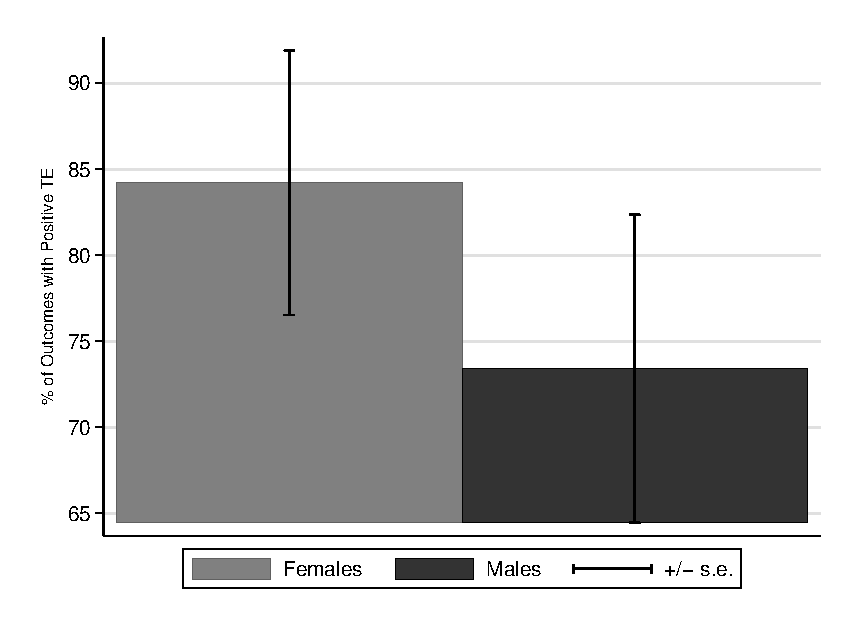
\includegraphics[width=\textwidth]{output/itt_noctrl_all.eps}
\end{subfigure}%
\begin{subfigure}[h]{0.4\textwidth}
	\centering
	\caption{Treatment vs. Next Best, Significant at 10\% Level} \label{fig:ppositive10}
		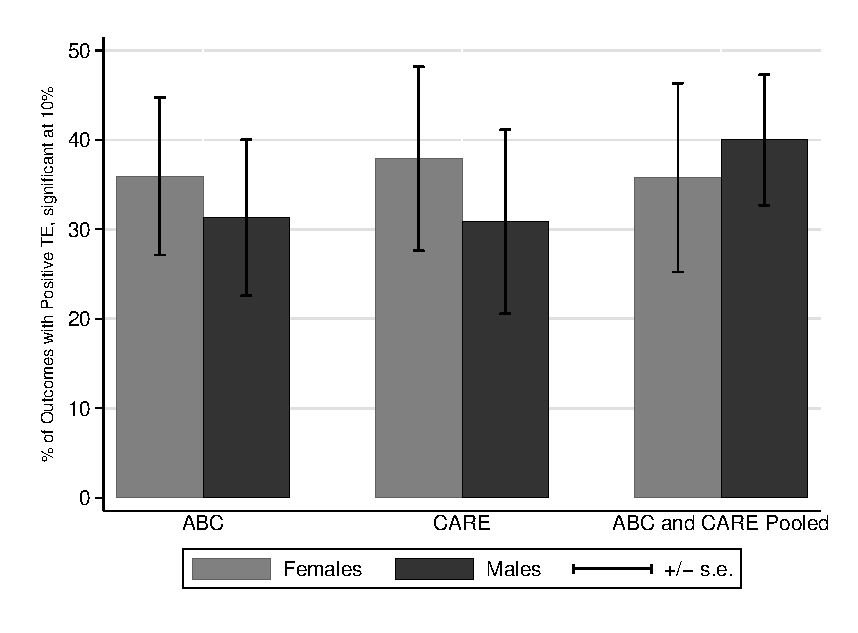
\includegraphics[width=\textwidth]{output/itt_noctrl_all_sig10.eps}
\end{subfigure}
\begin{subfigure}[h]{0.4\textwidth}
		\centering
		\caption{ Treatment vs. Stay at Home} \label{fig:ppositivehome}
		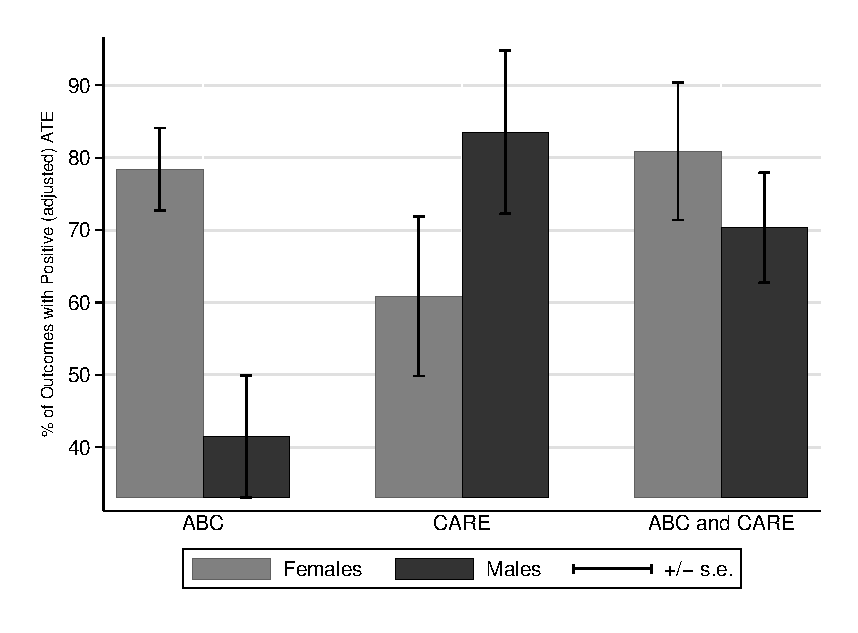
\includegraphics[width=\textwidth]{output/epan_ipw_p0_all.eps}
\end{subfigure}%
\begin{subfigure}[h]{0.4\textwidth}
	\centering
	\caption{Treatment vs. Alternative Preschool} \label{fig:ppositivealternative}
		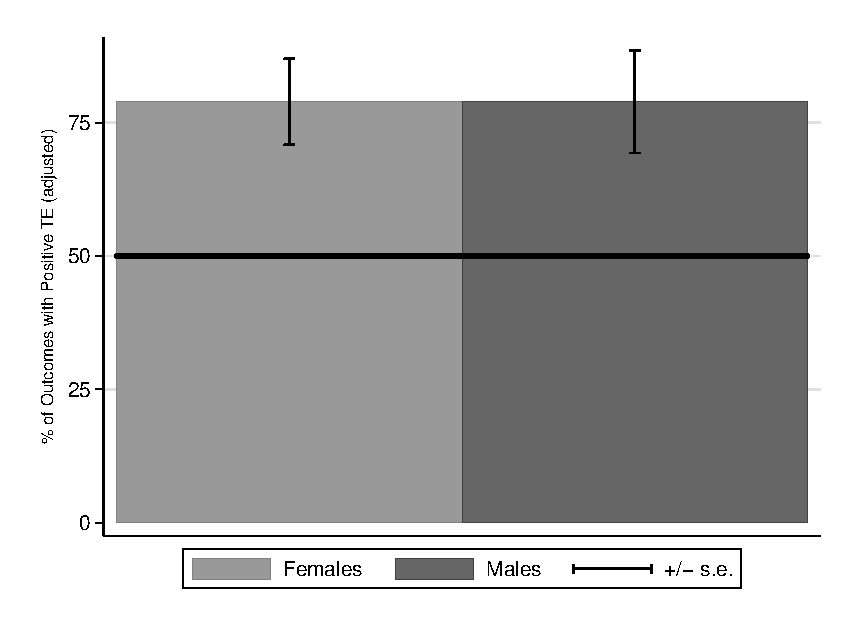
\includegraphics[width=\textwidth]{output/epan_ipw_p1_all.eps}
\end{subfigure}
\footnotesize \justify
Note: Panel (a) percentage of outcomes displaying a positive treatment effect, comparing treatment to next best. Panel (b) percentage of outcomes displaying a positive and statistically significant treatment effect (10\% significance level). Panel (c) displays the percentage of outcomes with a positive treatment effect, comparing treatment to staying at home. Panel (d) displays the percentage of outcomes with a positive treatment effect, comparing treatment to alternative childcare arranements. Standard errors are based on the empirical bootstrap distribution. For Panel (b) we perform a ``double bootstrap'' procedure to first determine significant treatment effects at $10\%$ level and then calculate the standard error of the count.\\
\end{sidewaysfigure}


\section{Predicting and Monetizing Life-cycle Costs and Benefits}\label{section:cbamethodology}

The major goal of this paper is to summarize the multiple benefits of ABC/CARE using benefit/cost and rate of return analyses. We rely on auxiliary data to predict the costs and benefits of the program over the life cycle after the measurement phase of the study ends.

We construct synthetic treatment and control cohorts.\footnote{See, e.g., \citet{Mincer_1974_schooling} and the survey in \citet{Heckman_Lochner_ea_2006_HEE}.} The problem in doing so comes in creating counterparts to the treatment and control groups in auxiliary samples. Outcomes of ``comparable'' older cohorts in auxiliary samples who are not exposed to the program are used to construct virtual treatment and control groups. We address the problem of finding who among the auxiliary samples would have received treatment if the program had been available to them.

In addition, older cohorts may have received different endowments and experienced different environments. An assumption of stationarity in life cycle profiles across cohorts may be grossly at odds with the data.

This section explains our strategy for constructing out-of-sample treatment effects. Our approach starts from and extends the analysis of \citet{Heckman_Pinto_etal_2013_PerryFactor}, who show, in a setting similar to ours, that the effect of treatment on outcomes operates through its effects on inputs in a stable production function rather than through shifts in the production function.
Table~\ref{table:sources} presents the outcomes for which we conduct these analyses and the data sources used. We initially focus on labor income to illustrate our approach, but a similar methodology is used to predict the other outcomes.

\begin{table}[!htbp]
\begin{threeparttable}
\caption{Auxiliary (Non-experimental) Data Sources for Interpolation and Extrapolation of Life-cycle Benefits and Costs} \label{table:sources}
\footnotesize
%\input{../../AuxilliaryFiles/Preamble}
%\newgeometry{margin=.1in}

%\newcolumntype{L}[1]{>{\raggedright\let\newline\\\arraybackslash\hspace{0pt}}m{#1}}
%\newcolumntype{C}[1]{>{\centering\let\newline\\\arraybackslash\hspace{0pt}}m{#1}}
%\newcolumntype{R}[1]{>{\raggedleft\let\newline\\\arraybackslash\hspace{0pt}}m{#1}}

\begin{tabular}{L{3cm} C{1cm} C{1cm} C{1cm} C{1cm} C{1cm} C{2cm}} \toprule
 & \multicolumn{6}{c}{Subject's Age} \\
\textbf{Component}  & 16--21 & 21--30 & 31--34 & 34--50 & 61--67 & 68--Death \\ \midrule
\textbf{Transfer Income} & & \multicolumn{1}{c}{\cellcolor[gray]{.8} cNLSY} & \multicolumn{3}{c}{\cellcolor[gray]{.7} NLSY79; PSID}  &  \\ \midrule
\textbf{Subject Income} & &  \multicolumn{1}{c}{\cellcolor[gray]{.8} cNLSY} & \multicolumn{3}{c}{\cellcolor[gray]{.7} NLSY79; PSID} & \\ \midrule
\textbf{Health}  & \multicolumn{6}{c}{\cellcolor[gray]{.8} PSID; MEPS; MCBS; HRS}     \\ \midrule
\textbf{Crime} & \multicolumn{4}{c}{\cellcolor[gray]{.8} NCDPS; NJRP; NVS; UCRS} \\ \bottomrule
\end{tabular}
%\end{document}
\begin{tablenotes}
\footnotesize
Note: This table presents the auxiliary data sources we use to interpolate and extrapolate the life-cycle benefits and costs of ABC/CARE. CNLSY: Children of the National Longitudinal Survey of the Youth 1979; NLSY79: National Longitudinal Survey of the Youth 1979; PSID: Panel Study of Income Dynamics; MEPS: Medical Expenditure Panel Survey; MCBS: Medicare Current Beneficiary Survey; HRS: Health and Retirement Study; NCDPS: North Carolina Department of Public Safety Data; NVS: National Crime Victimization Survey; NJRP: National Judicial Reporting Program; UCRS: Uniform Crime Reporting Statistics.
\end{tablenotes}
\end{threeparttable}
\end{table}


\subsection{Using Auxiliary Data Sources to Predict Out-of-Sample Outcomes}\label{sec:usingaux}

We first present an informal summary of our approach. The next section gives a formal justification and reports tests of key assumptions. The remaining sections give applications to other outcomes besides labor income.

We have data on control- and treatment-group members through age $a^{\ast}$. We can identify treatment effects within the experimental sample. We lack information on participant outcomes afterward. Post-$a^{\ast}$ treatment effects are required to construct counterfactual life-cycle profiles.

Making valid predictions of out-of-sample treatment effects does not require making valid predictions of separate out-of-sample treatment and control profiles. Only valid predictions of their difference is required.

Nonetheless, in this paper we focus on making valid predictions of separate treatment and control post-$a^*$ profiles. Doing so allows us to test the validity of our methodology by comparing (within the support of the experimental sample) outcomes for the experimental control and treatment groups with those from the synthetic control and treatment groups we generate.

Comparisons between the experimental control group and the synthetic control group are particularly compelling. By design, neither group receives treatment. In our data, all persons offered treatment accept it, so it is straightforward to construct synthetic control groups in auxiliary samples using only eligibility criteria.

We construct counterfactual profiles using a three-step procedure. In step 1, we use the experimental sample to conduct a dynamic mediation analysis relating the vector of outcomes at age $a$ ($\bm{Y}^{d}_{i,a}$) for $a\leq a^*$ to predictor variables (and interactions) that are affected by treatment ($\bm{X}^{d}_{i,a}$), as well as background variables ($\bm{B}$). It turns out that we accurately predict within-sample treatment effects as well as levels of treatment and control profiles using this approach. In step 2, we construct counterparts to treatment- and control-group members in the auxiliary samples. We compare these constructed counterparts to the actual samples for ages $a \leq a^\ast$. In step 3, we use the estimated dynamic relationships fit on the constructed samples to predict the post-$a^{\ast}$ outcomes.

We preview the outputs of this approach. Figure~\ref{fig:labor-income-profiles} displays the life-cycle labor income profiles predicted by our procedure for the treatment and control groups. It also compares the realized labor income to the model-predicted labor income at $a^*$. There is close agreement of the constructed profiles within sample. The pattern of life-cycle labor income we generate is typical for low-skilled workers \citep{Blundell-etal_2015_J-Pub-E,Gladden_Taber_2000_WageProgression,Sanders-Taber_2012_AR,Lagakos_Moll_etal_2016_LifeCycle_NBER}.\footnote{The prediction of labor (transfer) income is based on indicator variables of being male and being Black, mother's education, average PIAT scores from ages 5 to 7, years of education at age 30, income at age 21 and 30, and one-period lagged labor (transfer) income. We use labor income at age 21 to initialize this process. A justification for the use of these variables is in Appendix~\ref{appendix:methodology}.}

\begin{sidewaysfigure}[!htbp]
\centering
\caption{Predicted Labor Income Profiles for ABC/CARE Participants}\label{fig:labor-income-profiles}
\begin{subfigure}[h]{0.5\textwidth}
		\centering
		\caption{Males} \label{fig:labor-income-profilesc}
		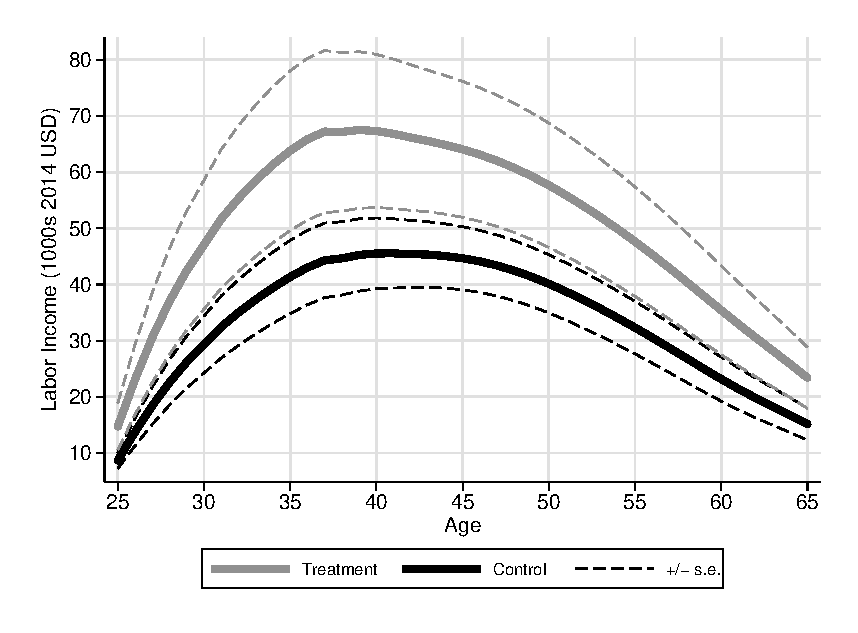
\includegraphics[width=\textwidth]{output/labor_25-65_pset1_mset3_male.eps}
\end{subfigure}%
\begin{subfigure}[h]{0.5\textwidth}
		\centering
		\caption{Females} \label{fig:labor-income-profilesa}
		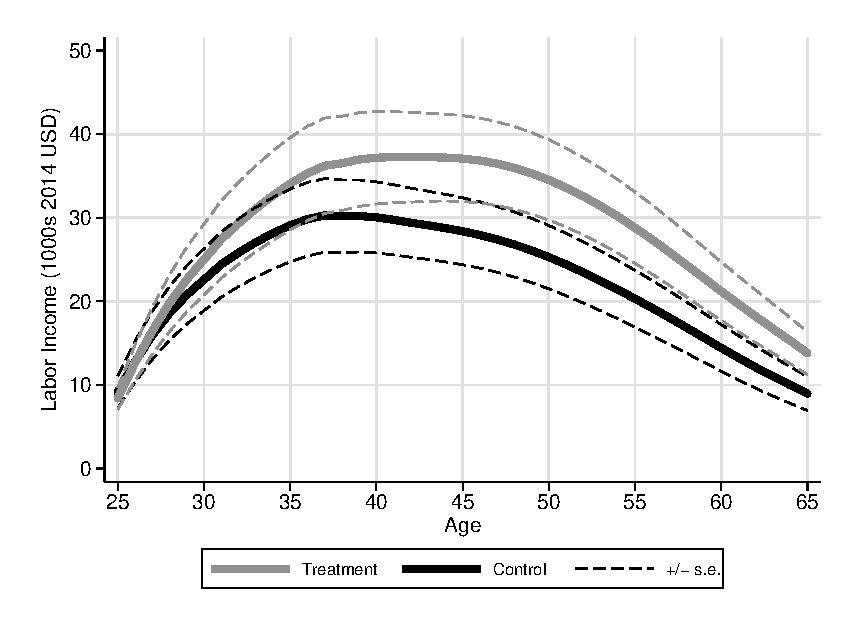
\includegraphics[width=\textwidth]{output/labor_25-65_pset1_mset3_female.eps}
\end{subfigure}
\footnotesize \justify
Note: Panel (a) displays the predicted life-cycle labor income profiles for ABC/CARE males by treatment status, based on the method proposed in this section. We combine data from the Panel Study of Income Dynamics (PSID), the National Longitudinal Survey of Youth 1979 (NLSY79), and the Children of the National Longitudinal Survey of Youth 1979 (CNLSY79). We highlight the \textit{observed} labor income at $a^*$ (age 30) for the ABC/CARE control- and treatment-group participants. Panel (b) displays the analogous figure for females. Our predictions go up to age 67, age of assumed retirement. Standard errors are based on the empirical bootstrap distribution. See Appendix~\ref{appendix:methodology} for a discussion of our choice of predictors and a sensitivity analysis of those predictors.
\end{sidewaysfigure}

We make a further check on the validity of our procedure. In the experimental sample all of the parents of children with characteristics $\bm{B} \in \mathcal{B}_0$ agree to participate in the program.  Because the auxiliary samples have no treatment group members, we can evaluate our procedure by comparing the labor incomes of individuals in the auxiliary samples for whom $\bm{B} \in \mathcal{B}_0$ to the labor incomes of individuals in our constructed synthetic control group. Figure~\ref{figure:controltests} makes this comparison. It plots the average labor incomes of individuals in our auxiliary sample for whom $\bm{B} \in \mathcal{B}_0$ alongside those of the constructed synthetic control group from ages 20 to 45. It also displays the labor income of the experimental control group at $a^*$ (age 30).\footnote{The graphs stop at age 45 because we do not observe all of the components of the risk index determinants of eligibility after age 45 in the auxiliary samples. We use only a subset of this index to make life-cycle projections. These variables are effective predictors over the age range for which the full set of $\bm{B}$ is available.} The agreement is reassuringly close. We now formalize our approach.

\begin{sidewaysfigure}[!htbp]
\centering
\caption{Labor Income Profile, Disadvantaged Individuals Synthetic Control Group in the Auxiliary Samples}\label{figure:controltests}
\begin{subfigure}[h]{0.5\textwidth}
		\centering
		\caption{Males}
		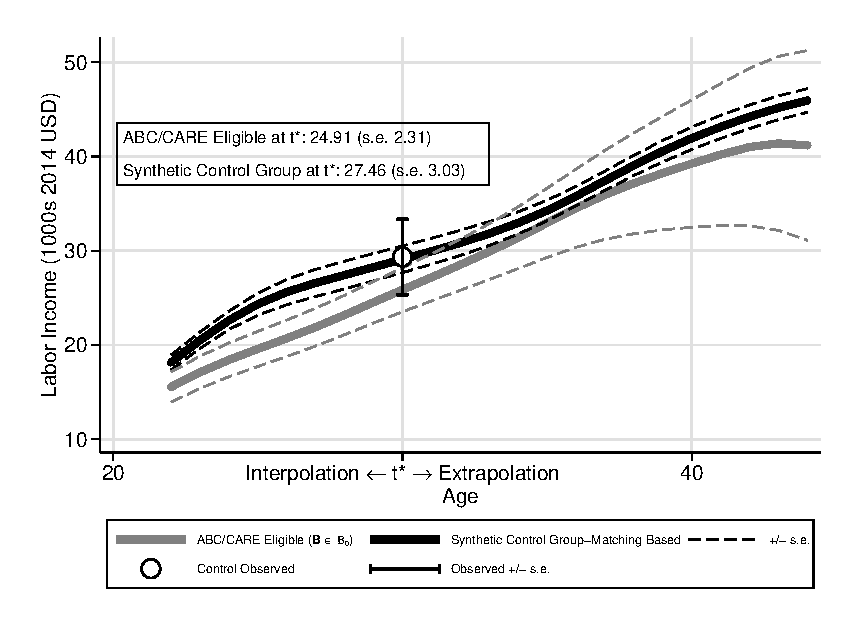
\includegraphics[width=\textwidth]{output/abccare_disad_1.eps}
\end{subfigure}%
\begin{subfigure}[h]{0.5\textwidth}
		\centering
		\caption{Females}
		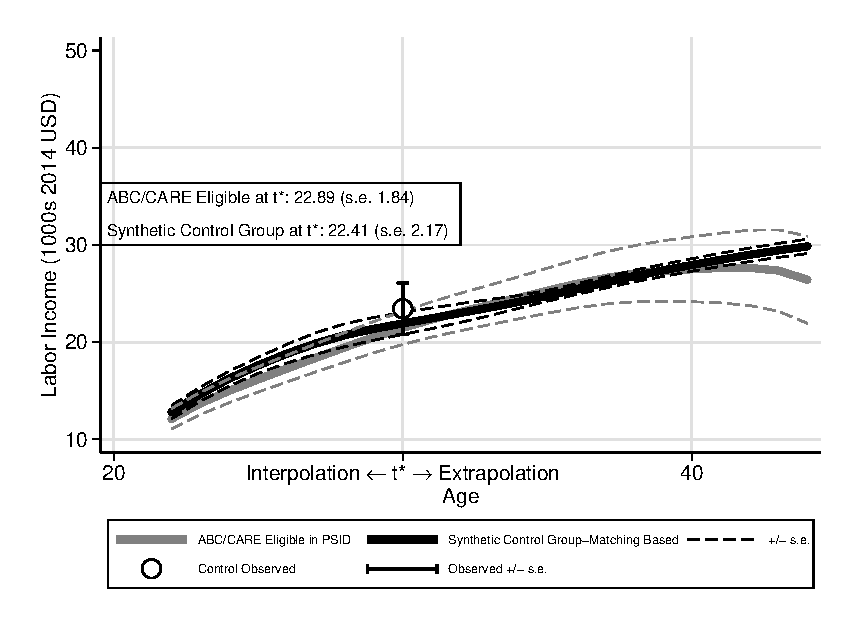
\includegraphics[width=\textwidth]{output/abccare_disad_0.eps}
\end{subfigure}
\footnotesize \justify
Note: Panel (a) displays the predicted labor income for males in the auxiliary samples for whom $\bm{B} \in \mathcal{B}_0$, i.e. ABC/CARE eligible, and for the synthetic control group we construct based on the method proposed in this section. We combine data from the Panel Study of Income Dynamics (PSID), the National Longitudinal Survey of Youth 1979 (NLSY79), and the Children of the National Longitudinal Survey of Youth 1979 (CNLSY79). We highlight the observed labor income at $a^*$ (age 30) for the ABC/CARE control- and treatment-group participants. We stop at age 45 for want of data to compute the High-Risk Index defining $\bm{B} \in \mathcal{B}_0$ in the auxiliary samples. Panel (b) displays the analogous figure for females. Standard errors are based on the empirical bootstrap distribution.
\end{sidewaysfigure}

\subsection{Constructing Out-of-Sample Counterfactuals}\label{section:just}

We now present our analytical framework and its underlying assumptions. Our analysis is based on a causal model for treatment ($d=1$) and control ($d=0$) outcomes for measure $j$ at age $a$ in sample $k \in \{e,n\}$ where $e$ denotes membership in the experimental sample and $n$ denotes membership in the control sample:
\begin{equation}\label{eq:outcome}
Y^d_{k,j,a} = \phi^d_{k,j,a} (\bm{X}^d_{k,a}, \bm{B}_k) + \varepsilon^d_{k,j,a}, \quad j \in \mathcal{J}_a.
\end{equation}
$\phi^d_{k,j,a}\left( \cdot, \cdot \right)$ is an invariant structural production relationship mapping inputs $\bm{X}^d_{k,a}, \bm{B}_k$ into output $Y^d_{k,j,a}$ holding error term $\varepsilon^d_{k,j,a}$ fixed.\footnote{Fixing and conditioning are fundamentally different concepts. See \cite{Haavelmo_1943_Econometrica} and \citet{Heckman_Pinto_2015_EconometTheory} for discussions. Our analysis applies the methodology in these papers.} We normalize $\varepsilon^d_{k,j,a}$ to have mean zero. Among the $\bm{X}^d_{k,a}$ are variables caused by treatment, including lagged dependent variables. The relationships between the dependent and right-hand side variables in \eqref{eq:outcome} do not necessarily coincide across the samples.

Let $\bm{Y}_k^d$ denote the vector of all outcomes at all ages for $k \in \{e, n \}$, when treatment status is fixed to $d$. Similarly, $\bm{X}_k^d$ is the vector of all causal predictors of $\bm{Y}_k^d$ at all ages. Both $\bm{Y}_k^d$ and $\bm{X}_k^d$ include the full set of possible outcomes over the life cycle, even though they are not sampled (observed) after age $a^*$. The background variables may have different distributions in the two samples. We denote the joint distribution of these vectors conditional on $\bm{B}_k = \bm{b}$ by $F_{\bm{Y}_k^d, \bm{X}_k^d | \bm{B}_k = \bm{b}}(\cdot,\cdot)$.

In the experimental sample, parents of eligible children ($\bm{B}_e \in \mathcal{B}_{0}$), always agree to participate in the program ($W_e = 1$) and accept treatment ($R_e = D_e$).\footnote{Thus, it is always true that $\bm{B}_e \in \mathcal{B}_{0}$ implies $W = 1$. Afterward, there are cases of attrition that could be interpreted as $R_e \neq D_e$, but this was not the case at the beginning of treatment. We distinguish attrition from non-compliance.} We assume that this condition holds in the auxiliary sample. Given this condition, we can use $D_e$ and $R_e$ interchangeably and apply a standard \citet{Quandt_1972_JASA} switching regression model to write the outputs and inputs generated by treatment as
\begin{spacing}{1}
\begin{align}\label{eq:countersystem}
Y_{k,j,a} =& \left( 1 - D_k \right) Y_{k,j,a}^0 + \left( D_k \right) Y_{k,j,a}^1, \\
&&j \in \mathcal{J}_a, a \in \{1,\dots,A\}, \quad k \in \{e,n\} \nonumber \\
\bm{X}_{k,a} =& \left( 1 - D_k \right) \bm{X}_{k,a}^0 + \left( D_k \right) \bm{X}_{k,a}^1. \nonumber
\end{align}
\end{spacing}

\noindent The fact that $D_e = R_e$ allows us to use experimental data (for $a \in \{1, \dots,a*\}$) to compute the distribution of $Y_{e,j,a}^d$ (i.e., $Y_{k,j,a}^d$ when fixing treatment status ($d$)).

\subsubsection{Accounting for Age, Period, and Cohort Effects}

The auxiliary data $(n)$ come from older cohorts not exposed to the program, for whom we observe more complete segments of their life cycles. We do not observe what treatment status $d$ would have been in the auxiliary data. Even if we did, we do not know if cohort ($c$) or time ($t$) effects make the experiences of the auxiliary-sample individuals different from the experiences of the individuals in the experimental sample.

To formalize this problem, and our solution to it, let $Y_{j,k,a,c,t}^d$ be outcome $j$ for sample $k$ at age $a$ for birth cohort $c$ at time $t$ when treatment is fixed to $d$. We make the following assumption. It amounts to avoiding the problem by saying cohort and time effects operate identically across the $e$ and $n$ samples in the following sense:

\onehalfspacing
\begin{assumption}\label{ass:alignment} \textbf{Alignment of Cohort and Time Effects}\\
For experimental sample cohort $c_{e}$ and auxiliary sample cohort $c_{n}$:
\begin{equation}
Y_{e,a,c_{e},t_{e}}^d = Y_{n,a,c_{n},t_{n}}^d
\end{equation}
for $d \in \{ 0, 1\}$, $a \geq a^*$, where $t_{e}, t_{n}$ are the years for which cohorts $c_{e}, c_{n}$ are observed, where $t_e = t_n + c_e - c_n$, and $t_n$ is the year the age $a$ outcome is observed for cohort $n$ ($t_n = a + c_n$). $\square$
\end{assumption}
\doublespacing

Notice that $Y^d_{n,a,{c_n},{t_n}}$ is the virtual outcome for treatment status $d$ in the auxiliary sample. This assumption does not rule out cohort or period effects. However, it rules out any \emph{differences} in cohort and time effects for the auxiliary group counterparts and the experimental groups when they reach the age of the auxiliary group.

We henceforth drop the ``$c$'' and ``$t$'' sub-indices. The out-of-sample year effect for the experimental sample is assumed to be the same as for the auxiliary sample counterpart measured at year $t_n$. We can weaken Assumption~\ref{ass:alignment} if there is prior knowledge about year and/or cohort effects or if we can parameterize estimable functions of $c$ and $t$.\footnote{See \cite{Heckman_Robb_1985_JE}.}

\subsubsection{Support Conditions}

In addition, we further require that the support of the auxiliary sample contains the support of the experimental sample. This assumption allows us to find counterpart values in the control and experimental samples.

\onehalfspacing
\begin{assumption} \label{ass:contain} \textbf{Support Conditions} \\
For $a \in \{ 1, \ldots, A \}$, the support of $\left( \bm{Y}^d_{e,a}, \bm{X}^d_{e,a}, \bm{B}_e \right)$ in the experimental sample is contained in the support of $\left( \bm{Y}^d_{n,t}, \bm{X}^d_{n,t}, \bm{B}_e \right)$ in the auxiliary sample:
\begin{equation}
supp( \bm{Y}_{e,a}, \bm{X}^d_{e,a}, \bm{B}_e ) \subseteq supp( \bm{Y}_{n,a}, \bm{X}^d_{n,a}, \bm{B}_n ), \quad d \in \{0,1\}. \quad \square
\end{equation}
\end{assumption}
\doublespacing
This assumption is straightforward to test for ages $a\leq a^\ast$. It is satisfied in our samples. See Appendix~\ref{app:containsupport}.

\subsubsection{Conditions for Valid Out-of-Sample Forecasts}

A strong sufficient condition for identifying the life-cycle profiles of individuals in the experimental sample using individuals in the auxiliary samples is Condition~\ref{cond:cond1}:

\onehalfspacing
\begin{condition} \textbf{Equality of Distributions Across the Experimental and Auxiliary Samples \label{cond:cond1}}
\begin{equation}
F_{\bm{Y}_e^d, \bm{X}_e^d | \bm{B}_e = \bm{b}} \left( \cdot, \cdot \right) = F_{\bm{Y}_n^d, \bm{X}_n^d | \bm{B}_n = \bm{b}} \left( \cdot, \cdot \right), \quad d \in \{0,1\}
\end{equation}
\noindent for $\bm{Y}_e^d, \bm{X}^d_e | \bm{B}_e = \bm{b}$ and $\bm{Y}_n^d, \bm{X}^d_n | \bm{B}_n = \bm{b}$ contained the support of the experimental sample $supp\left(\bm{Y}^d_{e,a}, \bm{X}^d_{e,a}, \bm{B}\right)$.
\end{condition}
\doublespacing

We are only interested in means for cost-benefit analysis. Thus, we can get by with Condition~\ref{cond:cond2}. It has testable implications, as we show below.

\onehalfspacing
\begin{condition} \textbf{Equality in Conditional Expectations Across the Experimental and Auxiliary Samples \label{cond:cond2}}
\begin{equation}
\mathbb{E} \left[ \bm{Y}_e^d |  \bm{X}_e^d = \bm{x}, \bm{B}_e = \bm{b} \right] = \mathbb{E} \left[ \bm{Y}_n^d |  \bm{X}_n^d = \bm{x}, \bm{B}_n = \bm{b} \right], \quad d \in \{0,1\}
\end{equation}
for $d \in \{0, 1 \}$ over $supp\left(\bm{Y}^d_{e,a}, \bm{X}^d_{e,a}, \bm{B}_e\right)$.
\end{condition}
\doublespacing

Since we are primarily interested in treatment effects, we can get by with an even weaker assumption:

\onehalfspacing
\begin{condition} \textbf{Equality in Mean Treatment Effects Across the Experimental and Auxiliary Samples \label{cond:cond3}}
\begin{equation}
\mathbb{E} \left[ \bm{Y}_e^1 - \bm{Y}_e^0 | \bm{B}_e = \bm{b} \right] = \mathbb{E} \left[ \bm{Y}_n^1 - \bm{Y}_n^0 | \bm{B}_n = \bm{b} \right]
\end{equation}
over $supp\left(\bm{Y}^d_{e,a}, \bm{B}_e\right)$.
\end{condition}
\doublespacing

\subsubsection{Exogeneity}

Conditions~\ref{cond:cond1}--\ref{cond:cond3} do not require that we take a position on the exogeneity of $\bm{X}^d_k, \: k \in \{e,n\}$. However, under exogeneity assumptions it is easier to use economic theory to generate and interpret treatment effects, to test the validity of our synthetic control groups, and to use matching to find auxiliary sample counterparts to treatments and controls. For these purposes, we assume:

\onehalfspacing
\begin{assumption}\label{ass:exog} \textbf{Exogeneity}\\
For all $a, a'' \in \{ 1, \ldots, A \}$ and for $d, d' \in \{0,1\}$,
\begin{equation}
\varepsilon^d_{k,j,t} \indep \bm{X}^{d^{\prime}}_{k,a^{''}} | \bm{B}_k = \bm{b}
\end{equation}
for all $\bm{b}$ in the support of $\bm{B}_k, \: k \in \{e,n\}$, for all outcomes $j \in \mathcal{J}_{a}$, where ``$\bm{M} \indep \bm{N}|\bm{Q}$'' denotes independence of $\bm{M}$ and $\bm{N}$ given $\bm{Q}$. $\square$
\end{assumption}
\doublespacing

\noindent We test this Assumption in Appendix~\ref{app:endogeneity}.

\subsubsection{Structural Invariance}

We assume that the variables $\bm{X}_{k,a}^d$ fully summarize treatment in the sense that any effect that treatment has on outcomes operates through the inputs $\bm{X}_{k,a}^d$ and not through shifts in the production function relating inputs to outputs (see \citealp{Heckman_Pinto_etal_2013_PerryFactor}). Assumption~\ref{ass:summary} formalizes this.

\onehalfspacing
\begin{assumption} \label{ass:summary} \textbf{Structural Invariance}\\
For all $\bm{x}, \bm{b} \in supp(\bm{X}^d_{e,a}, \bm{B}_e), k \in \{e,n\}$
\begin{align}
\phi_{k,j,a}^0 \left( \bm{x}, \bm{b} \right) &= \phi_{k,j,a}^1 (\bm{x}, \bm{b}) \\   \nonumber
                                                                     &=: \phi_{j,a} (\bm{x}, \bm{b}),
\end{align}
$\phi^d_{k,j,a}(\bm{x})$ is the function generating the causal effect of setting $\bm{X}^d_{k,a}=\bm{x}$ holding $\varepsilon^d_{k,j}$ fixed for $a \in \{1,\dots,A\}$ for any outcome $j \in \mathcal{J}_{a}$. $\square$
\end{assumption}
\doublespacing

This assumption has two messages that are fruitful to distinguish: (i) the structural functions evaluated at the same arguments have identical values for treatment and control groups in the experimental sample. It also says (ii) that the structural relationships are identical in the experimental and auxiliary samples. As previously noted, exogeneity is not needed to satisfy any of Conditions~\ref{cond:cond1} through \ref{cond:cond3}. But in the absence of exogeneity, the relationship between the $\bm{X}^d_{k,a}$ and the errors $\varepsilon^d_{k,a}$ likely differs across samples because the randomization imparts a source of exogenous variation to the $\bm{X}^d_{e,a}$ not present in the non-experimental sample. Assumption~\ref{ass:summary} combined with Assumption~\ref{ass:exog}, Equations~\eqref{eq:countersystem}, and the assumption of a zero mean for the errors $(\mathbb{E}(\varepsilon^d_{k,j,a})=0)$ for all $a \in \{1,\dots,A\}, d \in \{0,1\}$ and $k \in \{e,n\}$ enable us to write:
\begin{equation}\label{eq:invariancetest}
\mathbb{E} \left[ Y_{k,j,a}^d | \bm{X}_{k,a}^d  = \bm{x}, \bm{B}_k = \bm{b}, D = d \right] = \mathbb{E} \left[ Y_{k,j,a} | \bm{X}^d_{k,a}  = \bm{x}, \bm{B}_k = \bm{b} \right],
\end{equation}
for $a \in \{1,\dots,A\}$, $k \in \{e,n\}$, and $d \in \{0,1\}$.

\subsubsection{Testable Implications}

Equation~\eqref{eq:invariancetest} relates outcomes for $Y_{k,j,a}^d$ to treatment effects for $\bm{X}_{k,a}^d$, together with the background variables $\bm{B}_k$. It is possible to test \ref{ass:summary} within the experimental sample ($a \leq a^*$). The test consists of asking if $\bm{X}_{e,a}^d, \bm{B}$ predict the within experimental sample treatment effects for $Y_{e,j,t}$. Under the null hypothesis that \ref{ass:summary} is correct, a separate indicator variable for treatment status ($d$) is irrelevant when computing $\mathbb{E} \left[ Y_{e,j,a} | \bm{X}_{k,a}^d  = \bm{x}, \bm{B}_k =  \bm{b}, D = d \right]$. In Appendix~\ref{app:invariance}, we test and do not reject the null hypotheses.\footnote{This holds both when pooling males and females and when testing separately by gender (see Appendix~\ref{app:invariance}).}

Exogeneity and invariance enable us to test additional assumptions. By Equation~\eqref{eq:invariancetest}, we can write:
\begin{equation}\label{eq:withbetimplication}
\mathbb{E} \left[ Y_{e,j,a} | \bm{X}^d_{e,a} = \bm{x}, \bm{B}_e = \bm{b} \right] = \mathbb{E} \left[ Y_{n,j,a} | \bm{X}^d_{n,a} = \bm{x}, \bm{B}_e = \bm{b} \right], \quad d \in \{0,1\} \quad  a \in \{1,\dots,A\}.
\end{equation}
Relationship~\eqref{eq:withbetimplication} is testable for $a \leq a^*$, when $Y_{k,j,a}$ is observed in both the experimental and auxiliary samples. We do not reject the null hypotheses of no differences in the conditional mean functions in the experimental and auxiliary samples conditioning on $\bm{X}_{k,a}^d$ and $\bm{B}_k, \: k \in \{e,n\}$.\footnote{This holds when pooling males and females and when testing by gender (see Appendix~\ref{app:invariance}).}


\subsubsection{Summarizing the Implications of Exogeneity and Structural Invariance}

Collecting results, under exogeneity and structural invariance we obtain the following theorem:

\onehalfspacing
\setcounter{theorem}{0}
\begin{theorem}\label{theorem:main} \textbf{Valid Out-of-Sample Forecasts for Condition} \\
Under Assumptions~\ref{ass:alignment}-\ref{ass:summary}, Condition~\ref{cond:cond2} holds for any value of $\left( \bm{X}^d_{k,a}, \bm{B}_k \right)$. \\
\emph{This is an immediate consequence of the cited assumptions.} $\Box$
\end{theorem}
\doublespacing

\subsubsection{Testing for Endogeneity}\label{section:accendog}

In Appendix~\ref{app:endogeneity}, we investigate the question of endogeneity in the experimental and auxiliary samples. We follow \citet{Heckman_Pinto_etal_2013_PerryFactor} and assume that the $\varepsilon_{k,j,a}^d$ obey a factor structure, $k \in \{e,n\}$. We develop that framework and provide evidence supporting exogeneity in both samples for the variables used in our empirical analysis.

\subsubsection{Using Matching to Construct Virtual Treatment and Comparison Groups}

Under exogeneity assumption~\ref{ass:exog} and invariance condition~\ref{ass:summary} we can use matching to construct counterparts to treatment and control groups in the auxiliary sample.\footnote{\citet{Heckman_Ichimura_etal_1998_Econometrica} use this procedure.} We discuss this approach in Appendix~\ref{appendix:match}. Matching is one way to non-parametrically estimate the conditional mean functions. There is close agreement between non-parametric estimates based on matching and more parametric approaches (see Appendix~\ref{appendix:nonpar}).

\subsection{Predicting Parental Income} \label{section:pincome}

ABC/CARE offers childcare to the parents of treated children for more than nine hours a day for five years, 50 weeks a year. Only $27\%$ of mothers of children reported living with a partner at baseline and this status barely changed during the course of the experiment (see Appendix~\ref{appendix:background}). The childcare component generates the treatment effects in maternal labor force participation and parental income reported in Table~\ref{table:tescombined} and Appendix~\ref{appendix:results}.

We observe parental income at eight different time points for the experimental subjects up through age 21.\footnote{The ages at which parental income is observed is at ages 0, 1.5, 3.5, 4.5, 8, 12, 15, and 21. At age 21 the mothers in ABC/CARE were, on average, 41 years old.}$^,$\footnote{We linearly interpolate parental income for ages for which we do not have observations between 0 and 21.} As Table~\ref{table:tescombined} shows, treatment effects on parental income are sustained through the child's age 21. This presumably arises from wage growth due to parental attainment of further education and/or more work experience. An ideal approach would be to estimate the profile over the full life cycle of mothers. We propose two different approaches for doing this in Appendix~\ref{app:parentalincome}: (i) an approach based on parameterizing parental labor income using standard Mincer equations; and (ii) an approach based on the analysis of Section~\ref{section:just}. We present estimates using only the earnings through age 21 and using these two alternatives for projecting future earnings in Section~\ref{section:cbaresults}. The benefits of the program increase when considering the full life cycles of mothers using either approach.

Any childcare inducements of the program likely benefit parents who, at baseline, did not have any other children. If they did, then they might have had to take care of other children anyway, weakening the childcare-driven effect (especially if there are younger siblings present). In Appendix~\ref{app:endogeneity}, we show that the treatment effect for discounted parental income is much higher when there are no siblings of the participant children at baseline. The effect also weakens when comparing children who have siblings younger than 5 years old to children who have siblings 5 years old or younger.\footnote{These patterns persist when splitting the ABC/CARE sample by gender, but the estimates are not precise because the samples become too small. See Appendix~\ref{app:parentalincome}.}

\subsection{Health} \label{section:health}

We predict and monetize health outcomes based on a version of Equation~\eqref{eq:outcome} including a full vector of lagged dependent variables for different indicators of health status. This requires adapting the models of Section~\ref{section:just}. Three additional issues arise: (i) health outcomes such as diabetes or heart disease are absorbing states; (ii) health outcomes are highly interdependent within and across time periods; and (iii) there is no obvious terminal time period for benefits and costs except death, which is endogenous.\footnote{For example, for income we extrapolate up to the retirement age of 67. However, for health, we need to predict an age of death for each individual.}

Our auxiliary model for health is an adaptation of the Future America Model (FAM). This model predicts health outcomes from the subjects' mid-30s up to their projected death \citep{Goldman_etal_2015_Future-Elderly-Model-Report}.\footnote{The simulation starts at the age in which we observe the subject's age-30 follow-up.} Appendix~\ref{appendix:health} discusses the FAM methodology in detail. We initialize the health prediction model using the same variables that we use to predict labor and transfer income, along with the initial health conditions as listed in Table~\ref{table:transition}.

Our methodology has five steps: (i) estimate age-by-age health state transition probabilities using the Panel Study of Income Dynamics (PSID); (ii) match these transition probabilities to the ABC/CARE subjects based on observed characteristics; (iii) estimate quality-adjusted life year (QALY) models using the Medical Expenditure Panel Survey (MEPS) and the PSID; (iv) estimate medical cost models using the MEPS and the Medicare Current Beneficiary Survey (MCBS), allowing estimates to differ by health state and observed characteristics; and (v) predict the medical expenditure and QALYs that correspond to the simulated individual health trajectories.\footnote{As an intermediate step between (i) and (ii), we impute some of the variables used to initialize the FAM models (see Appendix~\ref{appendix:health}).}

Our microsimulation model starts with health predictions at age 30, along with the information on observed characteristics available at this age. Restricting it to the individuals for whom we have information from the age-34 health survey allows us to account for components that are important for predicting health outcomes. The models predict the probability of being in any of the states in the horizontal axis of Table~\ref{table:transition} at age $a+1$ based on the state at age $a$, which is described by the vertical axis of the table.\footnote{In practice, the predictions are based on two-year lags, due to data limitations in the auxiliary sources we use to simulate the FAM. For example, if the individual is 30 (31) years old in the age-30 interview, we simulate the trajectory of her health status at ages 30 (31), 32 (33), 34 (35), and so on until her projected death.} Absorbing states are an exception. For example, heart disease at age $a$ does not enter in the estimation of transitions for heart disease at age $a+1$ because it is an absorbing state: once a person has heart disease, she carries it through the rest of her life.

\begin{sidewaystable}[!htbp]
\begin{threeparttable}
\caption{Health State Transitions, Age $a$ as Predictor of Age $a+1$}\label{table:transition}
\scriptsize
\begin{tabular}{l|cccccccccccccc} \toprule
\multicolumn{1}{c}{Age $a$} & \multicolumn{14}{c}{Age $a+1$} \\ \midrule
  & Heart & Hyper- & Stroke & Lung  & Diabetes & Cancer & Disability & Mortality & Smoking  & Obesity & Health  & DI  & SS  & SSI  \\
&  Disease & tension &  & Disease & & & & &  &  & Insurance & Claim & Claim & Claim \\
Heart Disease & & & $\times$& & & &$\times$ &$\times$ & $\times$           &       &  $\times$  & $\times$ & $\times$ & $\times$\\
Hypertension  &  $\times$& & $\times$ & & & &$\times$ &$\times$ &       &     & $\times$   & $\times$ & $\times$  & $\times$\\
Stroke           & & & & & & &$\times$ &$\times$ &             &      &   $\times$  & $\times$ & $\times$  & $\times$\\
Lung Disease & & & & & & &$\times$ &$\times$ & $\times$         &        &   $\times$  &$\times$  & $\times$  & $\times$\\
Diabetes       & $\times$ &$\times$  & $\times$   & & & &$\times$ &$\times$ & $\times$            &       &  $\times$    & $\times$& $\times$ & $\times$ \\
Cancer         & & & $\times$ &  & &   &$\times$ & $\times$&           &         &   $\times$  & $\times$ & $\times$  & $\times$\\
Disability     & & & & & & &$\times$ &$\times$ &         &      &     $\times$  & $\times$ & $\times$   & $\times$\\
\midrule
Smoking & $\times$& $\times$&$\times$ & $\times$& $\times$& $\times$&$\times$ &$\times$ & $\times$   &   &     $\times$  & $\times$ & $\times$   & $\times$\\
BMI & $\times$& $\times$&$\times$ & $\times$& $\times$& $\times$&$\times$ & & $\times$    &  $\times$ &     &  &   & \\
Physical Activ. & $\times$& $\times$&$\times$ & $\times$& $\times$& $\times$&$\times$ & & $\times$    &   &     &   &  & \\
Binge Drinking & & & & & & &  &$\times$ & $\times$    &      &      &   &     &  \\
\midrule
DI Claim      & & & & &  & & & &             &         & $\times$    & $\times$   & $\times$ & $\times$\\
SS Claim     & & & & & & & &           &         &     & $\times$ &  & & $\times$\\
SSI Claim   & & & & &&  & & &         &        &      & &   & $\times$\\ \bottomrule
\end{tabular}

\begin{tablenotes}
\footnotesize
\item Note: This table illustrates how health outcomes at age $a$ predict health outcomes at age $a+1$. The crosses indicate if we use the age $a$ outcome to predict the age $a+1$ outcome. DI Claim: disability insurance claim; SS Claim: social security claim; DB Claim: disability benefits claim; SSI Claim: supplemental security income claim. The age $a$ states that do not predict themselves at age $a+1$ are absorbing states by construction.
\end{tablenotes}
\end{threeparttable}
\end{sidewaystable}

At each age, once we obtain the transition probability for each health outcome, we make a Monte-Carlo draw for each subject. Thus, each simulation depends on each individual's health history and on their particular characteristics. For every simulated trajectory of health outcomes, we predict the lifetime medical expenditure using the models estimated from the MEPS and the MCBS. We then obtain an estimate of the expected lifetime medical expenditure by taking the mean of each individual's simulated lifetime medical expenditure.

The same procedure is applied to calculate quality-adjusted life years (QALYs).\footnote{A quality-adjusted life year (QALY) reweighs a year of life according to its quality given the burden of disease. Suppose we assign a value of $\$150,000$ (2014 USD) to each year of life. A QALY of $\$150,000$ denotes a year of life in the absence of disease (perfect health). The value of QALY for an individual in a given year is smaller than $\$150,000$ when there is positive burden of disease, as worse health conditions imply lower QALYs. When an individual dies, her QALY equals zero. There are extreme combinations of disease and disability that may generate negative QALYs, although this is unusual.} We compute a QALY model based on a widely-used health-related Quality-of-life (HRQoL) measure (EQ-5D), available in MEPS.\footnote{For a definition and explanation of this instrument, see \citet{Dolan_1997_Modeling_MC,Shaw_etal_2005_EQ5D_MC}.} We then estimate this model using the PSID.

We estimate three models of medical spending: (i) Medicare spending (annual medical spending paid by parts A, B, and D of Medicare); (ii) out-of-pocket spending (medical spending paid directly by the individual); and (ii) all public spending other than Medicare. Each medical spending model includes the variables we use to predict labor and transfer income, together with current health, risk factors, and functional status as explanatory variables.

We also calculate medical expenditure before age 30. The ABC/CARE interviews at ages 12, 15, 21 and 30 have information related to hospitalizations at different ages and number of births before age 30. We combine this retrospective information and individual and family demographic variables with medical spending models estimates using MEPS to predict medical spending for each age.

QALYs are crucial for our benefit-cost analysis because they monetize the health of an individual at each age. Figure~\ref{fig:qalys} shows our estimation of QALYs together with a PSID comparison, in an exercise analogous to that used to produce Figure~\ref{fig:labor-income-profiles}.\footnote{In our baseline estimation, we assume that each year of life is worth  $\$150,000$ (2014 USD). Our estimates are robust to substantial variation in this assumption, as we show in Appendix~\ref{appendix:sensitivity}.} Although there is not a clear age-by-age treatment effect on QALYs, there is a significant difference in the accumulated present value of the QALYs between the treatment and the control groups. The QALYs for individuals in the control group match the QALYs of disadvantaged individuals in the PSID.\footnote{In Appendix~\ref{appendix:health} we further discuss and justify the parameterizations required to obtain estimates of QALYs. \citet{Goldman_etal_2015_Future-America-Model} examine the sensitivity to these parameterizations and discuss alternative micro-simulations monetizing health condition.}

\begin{figure}[!htbp]
\caption{Quality Adjusted Life Years, Predictions and Comparison to PSID}\label{fig:qalys}
\centering
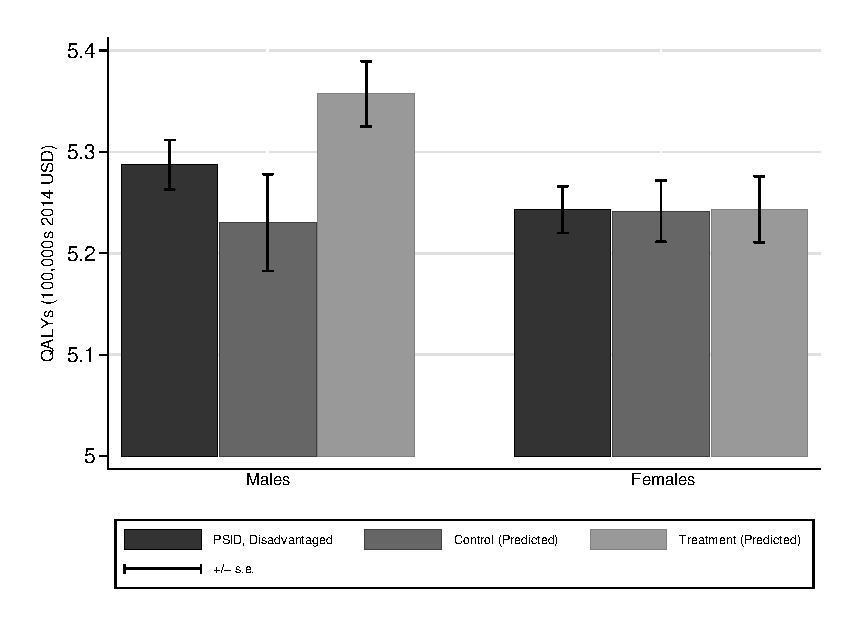
\includegraphics[width=.7\columnwidth]{output/qalyexppsid.eps}
\floatfoot{
\footnotesize
Note:  This figure displays the life-cycle net-present value of predicted quality-adjusted life years (QALYs) for ABC/CARE males and females, respectively, by treatment status. The predictions are based on combining data from the Panel Study of Income Dynamics (PSID), the Health Retirement Study, and the Medical Expenditure Panel Survey (MEPS). For each gender, we display a comparison to disadvantaged males and females in the Panel Study of Income Dynamics (PSID), where disadvantaged is defined as being Black and having 12 years of education or less. QALYs are the quality-adjusted life years gain due to better health conditions. Standard errors are based on the empirical bootstrap distribution.}
\end{figure}


\subsection{Crime\footnote{The input of Andr\'{e}s Hojman was essential for this component of our analysis.}}\label{sec:crime}

To estimate the life-cycle benefits and costs of ABC/CARE related to criminal activity, we use rich data on crime outcomes obtained from public police records.\footnote{Two previous studies consider the impacts of ABC on crime: \citet{Clarke_Campbell_1998_ABC_Comparison_ECRQ} use administrative crime records up to age 21, and find no significant differences between the treatment and the control groups. \cite{Barnett_Masse_2002_benefitcost,Barnett_Masse_2007_EER} account for self-reported crime at age 21. They find little effects, but the lack longer term, administrative data.} See Appendix \ref{appendix:crime} for a more complete discussion. We consider the following types of crime: arson, assault, burglary, fraud, larceny, miscellaneous (which includes traffic and non-violent drug crimes), murder, vehicle theft, rape, robbery, and vandalism. We use administrative data that document: (i) youth arrests, gathered at the age-21 follow-up; (ii) adult arrests, gathered at the age-34 follow-up; and (iii) sentences, gathered at the age-34 follow-up. We also use self-reported data on adult crimes, gathered in the age-21 and age-30 subject interviews. Because none of these sources capture all criminal activity, it is necessary to combine them to more completely approximate the crimes the subjects committed. We also use several auxiliary datasets to complete the life-cycle profile of criminal activity and compute the costs of the committed crimes.

We follow four steps to estimate the costs of crime.

\begin{enumerate}
\item \textit{Count arrests and sentences.} We start by counting the total number of sentences for each individual and type of crime (arson, assault, etc.) up to age 34, matching crimes across data sources, to construct the total number of  arrests for each individual and type of crime up to age 34.\footnote{In practice, we count all offenses (an arrest might include multiple offenses). This gives the correct number of victims for our estimations. The youth data have coarser categories than the rest of the data: violent, property, drug, and other. To match these data with the adult data, we assume that all property crimes were larcenies and that all violent crimes are assaults. In the ABC/CARE sample, assault is the most common type of violent crime, and larceny/theft is the most common property crime.} For individuals missing arrest data,\footnote{About 10\% of the ABC/CARE sample has missing arrest data. We fail to reject differences in observed characteristics between the treatment- and control-group participants for whom we observe arrests data (see Appendix~\ref{appendix:data}).} we impute the number of arrests by multiplying the number of sentences for each type of crime by a national arrest-sentence ratio for the respective crime.\footnote{This arrest-sentence ratio is constructed using the National Crime Victimization Survey (NJRP) and the Uniform Crime Reporting Statistics (UCRS).}

\item \textit{Construct predictions.} Based on the sentences observed before age 34, we predict the sentences that the ABC/CARE subjects will have after age 34. Data from the North Carolina Department of Public Safety (NCDPS), which provide lifetime sentences of individuals in North Carolina, are used to estimate sentences incurred after age 34 from sentences incurred before age 34. Applying these models to the ABC/CARE data, we predict the number of future sentences for each subject up to age 50.\footnote{We assume that individuals with no criminal records before age 34 commit no crimes after age 34.} We then add these estimates to the original number of sentences, getting an estimate of the lifetime sentences. Adding these estimates increases the total count of crimes by 30\%--50\%.

\item \textit{Estimate number of victims from the crimes.} We only observe crimes that resulted in consequences in the justice system: crimes that resulted in arrests and/or sentences. To include unobserved crimes, we use victimization inflation (VI).\footnote{Previous papers using this method include \citet{Belfield_Nores_etal_2006_JHR} and \cite{Heckman_Moon_etal_2010_RateofReturn}.} We start by constructing a VI ratio, which is the national ratio of victims and arrests for each type of crime.\footnote{We assume that each crime with victims is counted separately in the national reports on arrests, even for arrests that might have been motivated by more than one crime. This victim-arrest ratio is constructed using the NJRP and the National Crime Victimization Survey (NCVS).} Then, we estimate the number of victims from the crimes committed by ABC/CARE subjects as their total arrests multiplied by the VI ratio.\footnote{Additionally, we can calculate an analogous estimate of the number of crime victims using sentences, based on the VI ratio and the national arrests-to-sentences ratio. Both estimates are very similar, as shown in Appendix \ref{appendix:crime}. To improve precision, the estimates in the rest of our paper are based on the average of the two calculations.}

\item \textit{Find total costs of crimes.} We use the estimates of the cost of crimes for victims from \cite{McCollister_etal_2010_DAD} to impute the total victimization costs. For crimes resulting in arrests and/or sentences, we consider justice system costs as well, such as police costs.\footnote{To be able to assign costs to each type of crime, we assume that the cost of the justice system depends on the number of offenses of each type, rather than on the number of arrests. While this could very slightly overestimate justice system costs, the costs only represent about 5\% of the total crime costs.} Finally, we construct the total costs of incarceration for each subject using the total prison time and the cost of a day in prison.\footnote{Appendix~\ref{appendix:sensitivity} examines the sensitivity of our crime costs quantification to different assumptions. Section~\ref{section:cbaresults} and Appendix~\ref{appendix:sensitivity} we examine the sensitivity of our overall assessment of ABC/CARE results to the quantification of crime that we explain in this section.}
\end{enumerate}

\subsection{Education}

Follow-up data on educational attainment were collected through age 30. In Appendix \ref{appendix:education}, we show that using auxiliary data sources, education up to this age is an accurate predictor of lifetime educational attainment. Therefore, we do not predict educational attainment beyond age 30. To monetize the costs of education, we consider the public costs of K-12 education and the private costs of post-secondary education, including vocational programs and community college. Other costs of education include grade retention and special education. Previous analyses of ABC pay special attention to special education, arguing that savings due to a reduction in this category are substantial \citep{Barnett_Masse_2002_benefitcost,Barnett_Masse_2007_EER}.\footnote{Their analyses do not include CARE.} This category is much less important in our calculation.\footnote{Pooling males and females the net gain due to a reduction in special education is $\$9,724.4$ (2014 USD) (s.e. $\$8,608.1)$. For males the gain is $\$14,694.9$ (2014 USD) (s.e. $\$11,065.4$) and for females it is $4,077.5$ (2014 USD) (s.e. $\$14,892.0$). This quantity is discounted to child's birth.}

\section{Benefit/Cost Analysis} \label{section:cbaresults}

This section reports benefit/cost and rate of return analyses underlying Figure~\ref{figure:main}. Appendix~\ref{appendix:sensitivity} displays an extensive sensitivity analysis of each of the components we consider. It includes scenarios in which all our assumptions hold and scenarios in which they are drastically violated, providing bounds for our estimates.

\subsection{Program Costs} \label{section:programscosts}

The yearly cost of the program was \$18,514 per participant in 2014 USD. We improve on previous cost estimates using primary-source documents.\footnote{Our calculations are based on progress reports written by the principal investigators and related documentation recovered in the archives of the research center where the program was implemented. We display these sources in Appendix \ref{app:programcosts}. The main component is staff costs. Other costs arise from nutrition and services that the subjects receive when they were sick, diapers during the first 15 months of their lives, and transportation to the center. The control-group children also receive diapers during approximately 15 months, and iron-fortified formula. The costs are based on sources describing ABC treatment for $52$ children. We use the same costs estimates for CARE, for which there is less information available. The costs exclude any expenses related to research or policy analysis. A separate calculation by the implementers of the program indicates almost an identical amount (see Appendix~\ref{app:programcosts}).}

\subsection{Benefit/Cost Estimates}

Table~\ref{table:bcsens} presents our baseline estimates of benefit/cost ratios, Table~\ref{table:irrsens} presents the analogous internal rates of return. Pooling males and females, the results indicate that the program is socially efficient: the internal rate of return and the benefit/cost ratio are $12.3\%$ and $5.7$. \textit{The program generates a benefit of $5.7$ dollars for every dollar spent on it}. These estimates are statistically significant, even after accounting for sampling variation, serial correlation, and prediction error in the experimental and auxiliary samples and the tax costs of financing the program. These benefits arise despite the fact that ABC/CARE was much more expensive than other early childhood education programs---the treatment involved more services over a longer time period \citep{Elango_Hojman_etal_2016_Early-Edu}.

\newgeometry{top=.4in, bottom=.5in, left=.4in, right=.4in}
\begin{sidewaystable}[!htpb]
\begin{threeparttable}
\caption{Sensitivity Analysis for Benefit/Cost Ratios}
\label{table:bcsens}
\centering
\footnotesize
\begin{tabular}{>{\bfseries}lcc|cc|cc} \toprule
	&	\multicolumn{2}{c}{\textbf{\textit{Pooled}}}	&	\multicolumn{2}{c}{\textbf{\textit{Males}}}	&	\multicolumn{2}{c}{\textbf{\textit{Females}}}	\\ 
Baseline	&	\multicolumn{2}{c}{5.69 (s.e. 2.32)}	&	\multicolumn{2}{c}{11.62 (s.e. 5.49)}	&	\multicolumn{2}{c}{2.60 (s.e. 0.98)}	\\ \\
\multicolumn{7}{l}{\textit{Baseline: IPW and Controls, Life-span up to Age 79, Treatment vs. Next Best, 50\% Marginal tax 50\% (deadweight loss), Discount rate 3\%, Parental}} \\	
\multicolumn{7}{l}{\textit{income 0 to 21 (child's age), Labor Income predicted from 21 to 65, All crimes (full costs), Value of life 150,000.}} \\ \\ \midrule	
Specification	&	\textit{No IPW}	&	\textit{and No Controls}	&	\textit{No IPW}	&	\textit{and No Controls}	&	\textit{No IPW}	&	\textit{and No Controls}	\\
	&	\textbf{6.17}	&	\textbf{5.35}	&	\textbf{11.94} 	&	\textbf{10.74}	&	\textbf{2.91}	&	\textbf{2.79}	\\
	&	(2.35)	&	(2.04)	&	(6.14)	&	(4.12)	&	(0.97)	&	(0.81)	\\ \midrule
Prediction	&	\textit{to Age 21}	&	\textit{to Age 30}	&	\textit{to Age 21}	&	\textit{to Age 30}	&	\textit{to Age 21}	&	\textit{to Age 30}	\\
Span	&	\textbf{1.55}	&	2.01	&	\textbf{2.17}	&	2.80	&	1.17	&	1.52	\\
	&	(0.39)	&	(0.88)	&	(0.74)	&	(1.96)	&	(0.43)	&	(0.48)	\\ \midrule
Counter-	&	\textit{vs. Stay at Home}	&	\textit{vs. Alt. Presch.}	&	\textit{vs. Stay at Home}	&	\textit{vs. Alt. Presch.}	&	\textit{vs. Stay at Home}	&	\textit{vs. Alt. Presch.}	\\
factuals	&	\textbf{4.44}	&	\textbf{6.58}	&	3.88	&	\textbf{10.85}	&	\textbf{4.89}	&	\textbf{2.40}	\\
	&	(1.68)	&	(2.22)	&	(2.78)	&	(4.14)	&	(1.50)	&	(0.94)	\\ \midrule
Deadweight-	&	\textit{0\%}	&	\textit{100\%\textit}	&	\textit{0\%}	&	\textit{100\%\textit}	&	\textit{0\%}	&	\textit{100\%\textit}	\\
loss	&	\textbf{8.50}	&	\textbf{4.29}	&	\textbf{17.43}	&	\textbf{8.71}	&	\textbf{3.69}	&	2.06	\\
	&	(3.47)	&	(1.75)	&	(8.19)	&	(4.14)	&	(1.43)	&	(0.79)	\\ \midrule
Discount 	&	\textit{0\%}	&	\textit{7\%}	&	\textit{0\%}	&	\textit{7\%}	&	\textit{0\%}	&	\textit{7\%}	\\
Rate	&	13.38	&	2.40	&	29.50	&	4.21	&	5.34	&	1.43	\\
	&	7.01	&	0.80	&	15.93	&	1.88	&	3.81	&	0.37	\\ \midrule
Parental	&	\textit{Mincer Life-cycle}	&	\textit{Life-cycle Prediction}	&	\textit{Mincer Life-cycle}	&	\textit{Life-cycle Prediction}	&	\textit{Mincer Life-cycle}	&	\textit{Life-cycle Prediction}	\\
Income	&	\textbf{5.92}	&	\textbf{5.60}	&	\textbf{11.80}	&	\textbf{12.36}	&	\textbf{2.88}	&	\textbf{3.27}	\\
	&	(2.32)	&	(2.39)	&	(5.49)	&	(5.68)	&	(1.02)	&	(1.21)	\\ \midrule
Labor	&	\textit{.5\% Annual Decay}	&	\textit{.5\% Annual Growth}	&	\textit{.5\% Annual Decay}	&	\textit{.5\% Annual Growth}	&	\textit{.5\% Annual Decay}	&	\textit{.5\% Annual Growth}	\\
Income	&	\textbf{5.48}	&	\textbf{5.90}	&	\textbf{10.76}	&	\textbf{12.49}	&	\textbf{2.47}	&	\textbf{2.74}	\\
	&	(2.25)	&	(2.41)	&	(5.33)	&	(5.71)	&	(0.87)	&	(1.10)	\\ \midrule
Crime	&	\textit{Drop Major Crimes}	&	\textit{Halve Costs}	&	\textit{Drop Major Crimes}	&	\textit{Halve Costs}	&	\textit{Drop Major Crimes}	&	\textit{Halve Costs}	\\
	&	\textbf{5.14} 	&	\textbf{4.07}	&	\textbf{11.82}	&	\textbf{8.33}	&	\textbf{2.72}	&	2.25	\\
	&	(2.30)	&	(1.50)	&	(5.59)	&	(3.64)	&	(1.04)	&	(0.95)	\\ \midrule
Health	&	\textit{Drop All}	&	\textit{Double Value of Life}	&	\textit{Drop All}	&	\textit{Double Value of Life}	&	\textit{Drop All}	&	\textit{Double Value of Life}	\\
(QALYs)	&	\textbf{4.85}	&	\textbf{6.56}	&	\textbf{10.61}	&	\textbf{12.63}	&	\textbf{2.48}	&	2.73	\\
	&	(2.32)	&	(2.54)	&	(5.37)	&	(5.90)	&	(0.97)	&	(1.26)	\\ \bottomrule
\end{tabular} 
\begin{tablenotes}
\footnotesize
\item Note: This table displays sensitivity analysis of our baseline benefit/cost ratio calculation to the perturbations indexed in the different rows. The characteristics of the \textit{baseline} calculation are in the table header. IPW: adjusts for attrition and item non-response (see Appendix~\ref{app:method_partialobs} for details). Control variables: Apgar scores at ages 1 and 5 and a high-risk index (see Appendix~\ref{appendix:results} for details on how we choose these controls). When predicting up to ages 21 and 30, we consider all benefits and costs up to these ages, respectively. Counterfactuals: we consider treatment vs. next best (baseline), treatment vs. stay at home, and treatment vs. alternative preschools (see Section~\ref{section:methodsquestions} for a discussion). Deadweight loss is the loss implied by any public expenditure (0\% is no loss and 100\% is one dollar loss per each dollar spent). Discount rate: rate to discount benefits to child's age 0 (in all calculations). Parental income: see Appendix~\ref{app:parentalincome} for details on the two alternative predictions (Mincer and Life-cycle). Labor Income: .5\ annual growth (decay) is an annual wage growth (decay) due to cohort effects. Crime: major crimes are rape and murder; half costs takes half of victimization and judiciary costs. Health (QALYs): drop all sets the value of life equal to zero. Standard errors obtained from the empirical bootstrap distribution are in parentheses. Bolded $p$-values are significant at 10\%. For details on the null hypothesis see Table~\ref{table:cba}.
\end{tablenotes}
\end{threeparttable}
\end{sidewaystable}

\begin{sidewaystable}[!htpb]
\begin{threeparttable}
\caption{Sensitivity Analysis for Internal Rate of Return, ABC/CARE}
\label{table:irrsens}
\centering
\footnotesize
% matrix: allirr file: allirr_sens.tex  25 Sep 2016 09:11:16
\begin{table}[htbp]
\begin{tabular}{lcccccc} \hline \hline
 & pooled  & pooled  & males  & males  & females  & females  \\  \hline 
baseline &     0.087 &     0.052 &     0.138 &     0.048 &     0.126 &     0.048 \\  
specification &     0.092 &     0.087 &     0.147 &     0.148 &     0.136 &     0.122 \\  
. &     0.059 &     0.032 &     0.060 &     0.037 &     0.044 &     0.039 \\  
predictiontime &     0.099 &     0.127 &     0.110 &     0.127 &     0.104 &     0.115 \\  
. &     0.056 &     0.051 &     0.047 &     0.051 &     0.045 &     0.043 \\  
counterfactual &     0.131 &     0.089 &     0.085 &     0.162 &     0.100 &     0.132 \\  
. &     0.046 &     0.057 &     0.038 &     0.044 &     0.034 &     0.039 \\  
dwl &     0.128 &     0.068 &     0.175 &     0.118 &     0.174 &     0.103 \\  
. &     0.089 &     0.037 &     0.063 &     0.042 &     0.064 &     0.037 \\  
parental &     0.104 &         . &     0.148 &         . &     0.142 &         . \\  
. &     0.069 &         . &     0.053 &         . &     0.053 &         . \\  
lincome &     0.080 &         . &     0.127 &         . &     0.122 &         . \\  
. &     0.053 &         . &     0.054 &         . &     0.047 &         . \\  
crime &     0.089 &     0.081 &     0.153 &     0.122 &     0.124 &     0.110 \\  
. &     0.052 &     0.051 &     0.043 &     0.046 &     0.044 &     0.044 \\  
health &     0.091 &     0.085 &     0.136 &     0.134 &     0.112 &     0.127 \\  
. &     0.053 &     0.052 &     0.049 &     0.053 &     0.058 &     0.045 \\  
\hline \hline \end{tabular}
\end{table}

\begin{tablenotes}
\footnotesize
\item Note: This table displays sensitivity analysis of our baseline internal rate of return calculation to the perturbations indexed in the different rows. The characteristics of the \textit{baseline} calculation are in the table header. IPW: adjusts for attrition and item non-response (see Appendix~\ref{app:method_partialobs} for details). Control variables: Apgar scores at ages 1 and 5 and a high-risk index (see Appendix~\ref{appendix:results} for details on how we choose these controls). When predicting up to ages 21 and 30, we consider all benefits and costs up to these ages, respectively. Counterfactuals: we consider treatment vs. next best (baseline), treatment vs. stay at home, and treatment vs. alternative preschools (see Section~\ref{section:methodsquestions} for a discussion). Deadweight loss is the loss implied by any public expenditure (0\% is no loss and 100\% is one dollar loss per each dollar spent). Parental income: see Appendix~\ref{app:parentalincome} for details on the two alternative predictions (Mincer and Life-cycle). Labor Income: .5\ annual growth is an annual wage growth due to cohort effects; only benefit assumes labor income is the only benefit of the program. Crime: major crimes are rape and murder; half costs takes half of victimization and judiciary costs. Health (QALYs): drop all sets the value of life equal to zero. N/A: Standard errors obtained from the empirical bootstrap distribution are in parentheses. Bolded $p$-values are significant at 10\%. For details on the null hypothesis see Table~\ref{table:cba}.
\end{tablenotes}
\end{threeparttable}
\end{sidewaystable}
\restoregeometry
\doublespacing

We accompany these estimates with a set of sensitivity checks of statistical and economic interest. Our estimates are not driven by our methods for accounting for attrition and item non-response or by the conditioning variables we use when computing the net-present values. Although the internal rate of return remains relatively high when using participant outcome measures up to ages 21 or 30, the benefit/cost ratios indicate that accounting for benefits that go beyond age 30 is important. The return to each dollar is at most $3/1$ when considering benefits up to age 30 only (prediction span columns). Controlling for treatment substitutes available to controls also matters. Males benefit the most from ABC/CARE relative to attending alternative childcare centers, while females benefit the most from ABC/CARE relative to staying at home. We explore this difference below.

Our baseline estimates account for the deadweight loss caused by the government by taxing individuals to budget its expenditure for all government-related activities.\footnote{When the transaction between the government and an individual is a direct transfer, we consider .5 as a cost per each transacted dollar as we do not weight the final recipient of the transaction (e.g., transfer income). When the transaction is indirect, we classify it as government spending as a whole and consider its cost as 1.5 per each dollar spend (e.g. public education).} Our baseline estimate assumes that the marginal tax rate is $50\%$. Our estimates are robust to dropping it to $0\%$ or doubling it to $100\%$ (deadweight loss columns). Our baseline estimate of benefit/cost ratios is based on a discount rate of $3\%$. Not discounting roughly doubles our benefit/cost ratios, while they remain statistically significant using a higher discount rate of $7\%$ (discount rate columns).

Parental income is an important component of the benefit/cost ratio. We take a conservative approach in our baseline estimates and do not account for potential shifts in profiles in parental income due to education and work experience subsidized by childcare (see the discussion in Section~\ref{section:pincome}). This is based on observed parental income from when the ABC/CARE participants were ages 0 to 21.

Alternative approaches considering the gain for the parents through age 65 generate an increase in the gain due to parental income (parental income columns). As noted in Section~\ref{section:cbamethodology}, our estimates ignore any cohort effects. Individuals in ABC/CARE could experience positive cohort effects that might (i) make them more productive and therefore experience wage growth \citep{Lagakos_Moll_etal_2016_LifeCycle_NBER}; (ii) experience a negative shock such as an economic crisis and therefore experience a wage decline \citep{Jarosch_2016_JobSecurity_Econometrica}. Our estimates are robust when we vary annual growth and decay rates between $-.5\%$ to $.5\%$.

We do not conduct sensitivity analysis to investigate alternative plausible cohort effects of health costs. Treated individuals are healthier. They reduce medical costs. But they also live longer, increasing medical costs. These opposing effects tend to negate each other \citep{Goldman_etal_2015_Future-America-Model}. We have little guidance on predicting the future health costs and benefits of our cohort compared to the cohorts on which FAM is based.

We also examine the sensitivity of our estimates to (i) dropping the most costly crimes such as murders and rapes;\footnote{Two individuals in the treatment group committed a rape and one individual in the control group committed a murder.} and (ii) halving the costs of victimization and judiciary costs related to crime. The first sensitivity check is important because we would not want our calculation to be based on a few exceptional crimes. The second is important because victimization costs are somewhat subjective (see Appendix~\ref{appendix:crime}). Our benefit/cost analysis is robust to these adjustments, even when crime is a major component. Lastly, we examine the sensitivity with respect to our main health component: quality-adjusted life years. This is an important component because relatively healthier individuals survive longer and healthier, and treatment improves health conditions. It is important to note that this component largely accumulates later in life and therefore it is heavily discounted. Dropping the component or doubling the value of life does not have a major impact on our calculations.

\begin{table}[!htbp]
\centering
\caption{Cost/benefit Analysis of ABC/CARE, Summary}\label{table:cba}
\begin{threeparttable}
\scriptsize
\begin{tabular}{l r r r r r r r r r}																			
\toprule																			
&       \mc{3}{c}{Females}      &       \mc{3}{c}{Males}        &       \mc{3}{c}{Pooled}       \\																			
\cmidrule(lr){2-4}      \cmidrule(lr){5-7}      \cmidrule(lr){8-10}																			
Removed Component       &       NPV     &       IRR     &       B/C     &       NPV     &       IRR     &       B/C     &       NPV     &       IRR     &       B/C     \\																			
\midrule																			
None	&	161,759	&	\textbf{10.1\%}	&	\textbf{2.61}	&	919,049	&	\textbf{14.7\%}	&	\textbf{10.19}	&	636,674	&	\textbf{13.7\%}	&	\textbf{7.33}	\\
	&		&	(6\%)	&	(0.73)	&		&	(4\%)	&	(2.93)	&		&	(3\%)	&	(1.84)	\\ \\
Parental Income	&	148,854	&	4\%	&	1.12	&	107,907	&	\textbf{11\%}	&	\textbf{9.10}	&	116,953	&	\textbf{9\%}	&	\textbf{6.17}	\\
	&		&	(2\%)	&	(0.65)	&		&	(3\%)	&	(2.92)	&		&	(3\%)	&	(1.87)	\\
Subject Labor Income	&	41,908	&	9\%	&	\textbf{2.21}	&	238,105	&	\textbf{13\%}	&	\textbf{7.75}	&	133,032	&	\textbf{13\%}	&	\textbf{6.03}	\\
	&		&	(6\%)	&	(0.66)	&		&	(5\%)	&	(2.23)	&		&	(4\%)	&	(1.77)	\\
Subject Transfer Income	&	419	&	\textbf{10\%}	&	\textbf{2.61}	&	-7,265	&	\textbf{15\%}	&	\textbf{10.26}	&	-4,372	&	\textbf{14\%}	&	\textbf{7.38}	\\
	&		&	(6\%)	&	(0.73)	&		&	(4\%)	&	(2.93)	&		&	(3\%)	&	(1.84)	\\
Subject QALY	&	42,102	&	9\%	&	\textbf{2.20}	&	106,218	&	\textbf{14\%}	&	\textbf{9.14}	&	87,181	&	\textbf{13\%}	&	\textbf{6.48}	\\
	&		&	(6\%)	&	(0.69)	&		&	(6\%)	&	(2.73)	&		&	(5\%)	&	(1.79)	\\
Medical Expenditures	&	-16,037	&	9\%	&	\textbf{2.77}	&	-42,038	&	\textbf{15\%}	&	\textbf{10.61}	&	-31,221	&	\textbf{14\%}	&	\textbf{7.65}	\\
	&		&	(6\%)	&	(0.76)	&		&	(3\%)	&	(2.89)	&		&	(3\%)	&	(1.85)	\\
Alternative Preschools	&	16,691	&	8\%	&	\textbf{2.45}	&	13,434	&	\textbf{14\%}	&	\textbf{10.05}	&	14,659	&	\textbf{12\%}	&	\textbf{7.19}	\\
	&		&	(5\%)	&	(0.73)	&		&	(4\%)	&	(2.92)	&		&	(3\%)	&	(1.84)	\\
Education Costs	&	1,457	&	\textbf{10\%}	&	\textbf{2.59}	&	-7,852	&	\textbf{15\%}	&	\textbf{10.26}	&	-4,518	&	\textbf{14\%}	&	\textbf{7.37}	\\
	&		&	(6\%)	&	(0.72)	&		&	(4\%)	&	(2.93)	&		&	(3\%)	&	(1.86)	\\
Crime Costs	&	31,668	&	10\%	&	\textbf{2.34}	&	638,923	&	\textbf{9\%}	&	4.08	&	450,368	&	\textbf{8\%}	&	\textbf{3.06}	\\
	&		&	(6\%)	&	(0.62)	&		&	(5\%)	&	(2.18)	&	&	(4\%)	&	(1.01)	\\ \\
Deadweight Loss	&		&	\textbf{18\%}	&	\textbf{3.83}	&		&	\textbf{19\%}	&	\textbf{15.38}	&		&	\textbf{18\%}	&	\textbf{11.01}	\\
	&		&	(12\%)	&	(1.04)	&		&	(6\%)	&	(4.35)	&		&	(5\%)	&	(2.79)	\\
0\% Discount Rate	&		&		&	\textbf{5.06}	&		&		&	\textbf{25.45}	&		&		&	\textbf{17.40}	\\
	&		&		&	(2.82)	&		&		&	(10.42)	&		&		&	(5.90)	\\
7\% Discount Rate	&		&		&	\textbf{1.49}	&		&		&	\textbf{3.78}	&		&		&	\textbf{2.91}	\\
	&		&		&	(0.32)	&		&		&	(0.79)	&		&		&	(0.59)	\\
\bottomrule																			
\end{tabular}																			

\begin{tablenotes}
\footnotesize
\item Note: This table presents the estimates of the net present value (NPV) for each component, and the internal rate of return (IRR) and the benefit/cost ratio (B/C) of ABC/CARE for different scenarios based on comparing the groups randomly assigned to receive center-based childcare and the groups randomly assigned as control in ABC/CARE. The first row represents the baseline estimates. The rest of the rows present estimates for scenarios in which we remove the NPV estimates of the component listed in the first column. Alternative Preschools refer to money spent in alternatives to treatment from the control-group children parents. QALYs refers to the quality-adjusted life years. Any gain corresponds to better health conditions through age death. The quantity listed in the NPV columns is the component we remove from NPV when computing the calculation in each row. All the money figures are in 2014 USD and are discounted to each child's birth, unless otherwise specified. For the B/C we use a discount rate of $3\%$, unless otherwise specified. We test the null hypotheses $\text{IRR} = 3\%$ and $\text{B/C} = 1$---we elect $3\%$ because that is the discount rate we use. Inference is based on non-parametric, one-sided $p$-values from the empirical bootstrap distribution. We highlight point estimates significant at the $10\%$ level.\\
    Total cost of the program per child is $92,570$.
\end{tablenotes}
\end{threeparttable}
\end{table}

The estimates are robust when we conduct a drastic sensitivity analysis by removing components of the benefit/cost analysis entirely (Table~\ref{table:cba}).\footnote{In Appendix~\ref{appendix:sensitivity}, we present exercises that are not as drastic as removing the whole component, but instead removing fractions of it.} Even when completely removing the gain associated with crime for males, the program is socially efficient---both the internal rate of return and the benefit/cost ratio are substantial. Parental income and crime are the components for which the internal rate of return and the benefit/cost ratio are the most sensitive. The reason for the sensitivity to parental income is that the amount is substantial and it is not heavily discounted because it accumulates during the first $21$ years of the children's life.\footnote{Depending on views about choice of individuals in labor markets, parental income should be excluded or included. If markets are neoclassical, the marginal value of foregone leisure is the wage and our our measure of parental income overstates the benefits of working. If nonemployment is involuntary, the full benefits should be counted.} Crime occurs later in life and its benefits are discounted accordingly. The amount due to crime savings is large so removing it diminishes both the internal rate of return and the benefit/cost ratio (but they remain statistically significant).

\textit{Our sensitivity analyses indicate that no single category of outcomes drives the social efficiency of the program. Rather, it is the life-cycle benefits across multiple dimensions of human development.}

In Appendix~\ref{appendix:bcaestimates} we use our analysis to examine the empirical foundations of recent cost-benefit studies of early childhood programs that use short term estimates of experimental test score gains coupled with auxiliary estimates of the impact of test scores on earnings (see, e.g., work by \citealp{Kline_Walters_2016_QJE}). We show that this approach applied to the ABC data greatly understates the true benefit-cost ratio because (a) earnings are only forecast through a young age (27) and (b) benefits extend beyond earnings. The difference is sizable. Applying the Kline and Walters method to the ABC/CARE experiment, we would find a cost-benefit ratio of 1.4 compared to our estimate of 5.7.

\begin{sidewaysfigure}[!htbp]
\centering
\caption{Life-cycle Net Present Value of Main Components of the CBA}\label{fig:npvsgender}
\begin{subfigure}[h]{0.5\textwidth}
		\centering
		\caption{Males}
		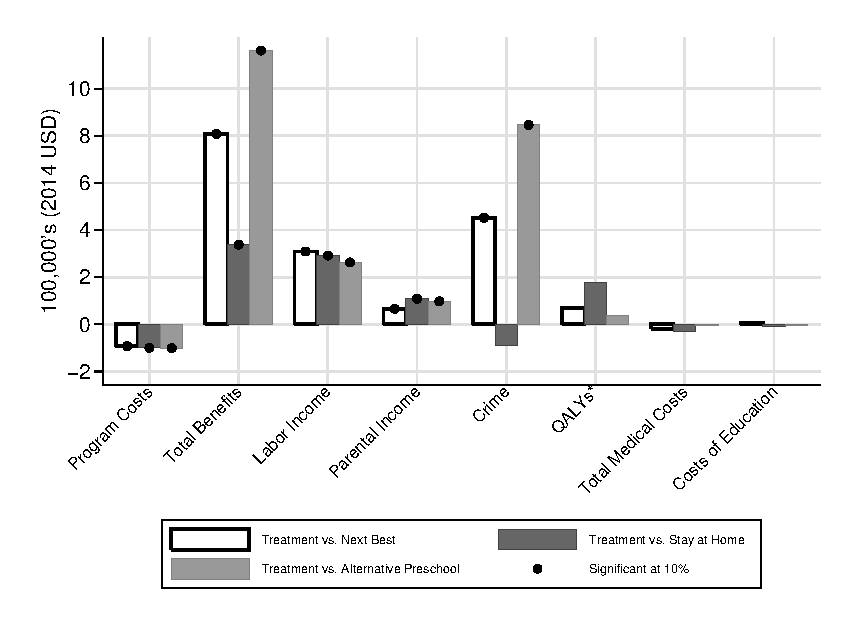
\includegraphics[width=\textwidth]{output/abccare_npvs2.eps}
\end{subfigure}%
\begin{subfigure}[h]{0.5\textwidth}
		\centering
		\caption{Females}
		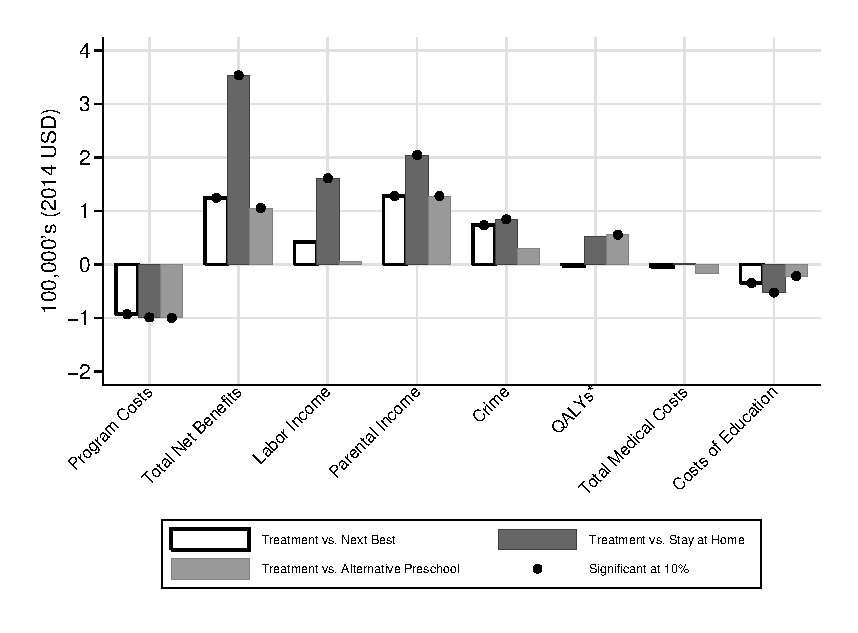
\includegraphics[width=\textwidth]{output/abccare_npvs1.eps}
\end{subfigure}
\footnotesize \justify
Note: This figure displays the life-cycle net present values of the main components of the cost/benefit analysis of ABC/CARE from birth to predicted death, discounted to birth at a rate of 3\%. ``Treatment vs. Control'': compares the treatment to the control group. ``Treatment vs. Stay at Home'': compares the treatment group to those subjects who stayed at home. ``Treatment vs. Alternative Preschool'': compares the treatment group to those subjects who attended alternative preschools. The latter two are based on matching estimators that account for selection on observable variables. By ``net" we mean that each component represents the total value for the treatment group minus the total value for the control group. Program costs: the total cost of ABC/CARE, including the welfare cost of taxes to finance it. Total net benefits: are for \textit{all} of the components we consider. These include labor income: total individual labor income from ages 20 to the retirement of program participants (assumed to be age 67). Parental income: total parental labor income of the parents of the participants from when the participants were ages 1.5 to 21. Crime: the total cost of crime (judicial and victimization costs). To simplify the display , the following components are not shown in the figure: (i) cost of alternative preschool paid by the control group children parents; (ii) the social welfare costs of transfer income from the government; (iii) disability benefits and social security claims; (iv) costs of increased individual and maternal education (including special education and grade retention); (v) total medical public and private costs. Inference is based on non-parametric, one-sided $p$-values from the empirical bootstrap distribution. We indicate point estimates significant at the $10\%$ level.\\
*The treatment vs. stay at home net present value is sizable and negative (-\$91,476.3); its standard error is \$86,657.3.\\
**QALYs refers to the quality-adjusted life years. Any gain corresponds to better health conditions until predicted death, with $\$150,000$ (2014 USD) as base value for a year of life.\\
\end{sidewaysfigure}

\subsection{Possible Explanations for Gender Differences}

The benefit/cost ratio and internal rate of return calculations both indicate that males and females benefit \emph{differently} from the program compared to the alternatives ``$H$'' and ``$C$''. There are two complementary stories that explain this difference. First, we explore reasons why the differences could exist if we simply consider the outcomes we are monetizing, and not the particular counterfactuals we estimate. Males have relatively high benefits from outcomes that we are able to monetize: labor income and crime are two examples of this. Historically, females are less likely to work than males. While all males supply labor in our sample at age 30, not all females supply labor. We are not able to quantify household production benefits for either males or females. This is an important omission for females who decide to stay at home instead of working.

Males are much more likely to commit crimes that are more costly to the victims and to the criminal justice system \citep{Cohen-Bowles_2010_Estimating-Cost-Crime,Gregg_etal_2015_SocialRealities_BOOK}. ABC/CARE also has treatment effects on crime for females for a number of categories (see Appendix~\ref{appendix:results}). However, males commit crimes that are much more expensive. These two categories are examples of why the magnitudes of the gains are much higher for males than they are for females.

For health, there are also substantial gender differences. Both males and females have substantial gains: males on more standard measures of physical health, while females on a set of mental health measures (see Appendix~\ref{appendix:results}). We quantify both components (see Section~\ref{section:health} and Appendix~\ref{appendix:health}).

When analyzing different counterfactuals, there is a substantial difference between males and females. The difference is driven by one of the counterfactuals: treatment vs. alternative preschools. The estimates for both males and females generate a similar estimated ABC/CARE treatment effect compared to staying at home. Males benefit much more from treatment relative to alternative preschools compared to their benefits from treatment relative to staying at home. This result is consistent with findings noted elsewhere: (i) stark gender differences resulting from attending low quality childcare \citep{Kottelenberg-Lehrer_2014_Gender-Effects,Baker_Gruber_Milligan_2015_Noncog_Defects}; and (ii) females are less sensitive to uncertain environments \citep{Autor-etal_2015_Family-Disadvantage}. The program substantially reduced the costs of special education for boys.

Our evidence does not indicate that the program has no benefit for females. In fact it does. When compared to staying at home, there is a gain of $4.81$ dollars per each dollar invested. When we decompose the net-present value for each of the components that we monetize, we find substantial benefits for females across a variety of categories, including health and crime. For males, the magnitudes are noticeably increased when comparing treatment to alternative preschool (see Figure~\ref{fig:npvsgender}).

\section{Summary} \label{section:conclusion}

This paper studies two influential early childhood programs evaluated by the method of randomized control trials with long term follow up through age 34. These programs are emulated in a variety of active early childhood programs around the world. We document outcomes across multiple life domains. We find an aggregate benefit/cost ratio of $5.7$ and a rate of return of $12.3\%$ per annum, even after adjusting for welfare costs of financing the program through public revenue.

To reach these conclusions, we address a number of empirical challenges: (a) control group substitution; (b) extrapolating lifetime benefits beyond the experimental period; and (c) the multiplicity of hypotheses tested. Our approach serves as a template for economic evaluations of programs with partial follow up over the life cycle.

Benefits differ substantially by gender. Females have more beneficial treatment effects than males, but the monetized value of the male treatment effects is greater. There are substantial effects on health and (health-related) quality of life and on crime for males. For females, the benefits are concentrated on education, employment, and minor crimes. The effects for females are stronger compared to the alternative of staying at home. The effects for males are stronger compared to the alternative of participation in alternative childcare arrangements. The program subsidizes maternal employment and has a strong causal effect on maternal labor income. We establish the benefits of analyzing long term multiple benefits of these programs.

%References
\singlespace
\bibliographystyle{chicago}
\bibliography{heckman}

\end{document} 